\documentclass[conference]{IEEEtran}
\IEEEoverridecommandlockouts
% The preceding line is only needed to identify funding in the first footnote. If that is unneeded, please comment it out.
\usepackage{amsmath}
\usepackage{amssymb}
\usepackage{array}
\usepackage{booktabs}
\usepackage{cite}
\usepackage{graphicx}
\usepackage{hyperref}
\usepackage{url}
\usepackage{xcolor}

\graphicspath{{../figures/}{figures/}}
\newcommand{\atk}[2]{\textbf{#1}~#2}
\newcommand{\emptycell}{--}
\definecolor{ptM}{HTML}{FF6B6B}
\definecolor{ptO}{HTML}{FFD166}
\definecolor{ptG}{HTML}{F4E04D}
\definecolor{ptU}{HTML}{4DABF7}
\definecolor{ptB}{HTML}{B197FC}
\definecolor{ptD}{HTML}{74C0FC}
\definecolor{ptS}{HTML}{63E6BE}
\definecolor{ptR}{HTML}{8CE99A}
\definecolor{ptN}{HTML}{69DB7C}
\definecolor{ptP}{HTML}{F783AC}
\newcommand{\ptile}[4]{\fcolorbox{black!35}{#1}{\begin{minipage}[c][0.44in][c]{0.92in}\centering{\large\bfseries #2}\\[-1pt]{\scriptsize #3}\\[-2pt]{\tiny #4}\end{minipage}}}
\newcommand{\btile}{\fcolorbox{black!10}{white}{\begin{minipage}[c][0.44in][c]{0.92in}\end{minipage}}}

\title{Supplement for A Periodic Table of Data Poisoning}
\author{
\IEEEauthorblockN{Yulia Kumar}
\IEEEauthorblockA{\textit{Department of Comp. Science and Technology, Kean University} \\
\textit{Department of ECE, Rutgers University}\\
Union, NJ and Piscataway, NJ \\
ykumar@kean.edu}
\and
\IEEEauthorblockN{Armando Luna}
\IEEEauthorblockA{\textit{Department of Comp. Science and Technology} \\
\textit{Kean University}\\
Union, NJ \\
lunaarm@kean.edu}

\and
\IEEEauthorblockN{Dov Kruger}
\IEEEauthorblockA{\textit{Department of Electrical and Computer Engineering} \\
\textit{Rutgers University}\\
Piscataway, NJ \\
Dov.Kruger@rutgers.edu}
\and
\IEEEauthorblockN{J. Jenny Li}
\IEEEauthorblockA{\textit{Department of Comp. Science and Technology} \\
\textit{Kean University}\\
Union, NJ \\
juli@kean.edu}
}

\begin{document}
\maketitle




\section{Current Results}


This supplement lists the detailed artifacts that are not printed as standalone objects in the six-page main paper. The main paper keeps the compact taxonomy tables, dataset summaries, metric definition, and food-image summary; the supplement preserves the method-level rows, split plots, examples, model notes, fidelity notes, and generated-output inventory.

\begin{table*}[t]
\centering
\caption{Supplement artifact inventory. Items listed here are repository artifacts not printed as standalone objects in the main six-page paper.}
\label{tab:suppartifactinventory}
\small
\begin{tabular}{p{0.28\textwidth}p{0.18\textwidth}p{0.46\textwidth}}
\toprule
Artifact or file group & Status & Purpose \\
\midrule
\texttt{fungi/fish/seafood\_attack\_comparison\_split.png} & Embedded & Stage-separated poisoning and evasion analog plots. \\
\texttt{fungi/fish/seafood\_attack\_examples.png} & Embedded & Representative clean, perturbed, and patch-trigger images. \\
\texttt{fungi\_reporting\_dashboard.png} & Embedded & Dashboard view of effects, clean accuracy, risk levels, and perturbation footprint. \\
\texttt{attack\_success\_by\_stage.png} & Listed & Cross-dataset mean normalized effect summary for fungi, fish, and seafood. \\
\texttt{*\_attack\_comparison\_bars.png}, \texttt{fungi\_dataset\_split.png} & Listed & Alternate generated bar and split sanity-check figures. \\
\texttt{periodic\_table\_data\_poisoning.png/.svg}, \texttt{paper\_taxonomy\_panels.png} & Listed & Poster and paper-oriented taxonomy exports; the main paper uses native LaTeX tables. \\
\texttt{results/*.csv}, \texttt{results/*.json}, \texttt{results/*.md} & Listed & Source rows, citation checks, implementation coverage, layout audit, and seafood duplicate audit. \\
\bottomrule
\end{tabular}
\end{table*}

\begin{table*}[t]
\centering
\caption{Fungi comparison table. Poisoning rows retrain MobileNetV3-Small; evasion rows attack the clean baseline.}
\label{tab:results}
\small
\begin{tabular}{p{0.25\textwidth}p{0.06\textwidth}p{0.05\textwidth}p{0.10\textwidth}p{0.28\textwidth}p{0.08\textwidth}}
\toprule
Method & Stage & Risk & Clean acc. & Metric & Value \\
\midrule
Clean baseline & Ref. & -- & 0.6667 & Poisonous \(\rightarrow\) edible confusion & 0.2708 \\
Random label flip & Poison & R3 & 0.5778 & Clean accuracy drop & 0.0889 \\
Targeted label flip & Poison & R2 & 0.7111 & Poisonous \(\rightarrow\) edible confusion & 0.3125 \\
Subpopulation label poison & Poison & R2 & 0.5667 & Selected subgroup \(\rightarrow\) edible & 0.6842 \\
BadNets patch backdoor & Poison & R1 & 0.5778 & Trigger ASR to edible & 0.2941 \\
Clean-label patch backdoor & Poison & R1 & 0.6111 & Trigger ASR to edible & 0.1714 \\
Sleeper-Agent-style backdoor & Poison & R1 & 0.5667 & Stealth-trigger ASR to edible & 0.6296 \\
Clean-label Poison Frogs & Poison & R1 & 0.6333 & Poisonous \(\rightarrow\) edible confusion & 0.3542 \\
Witches' Brew gradient match & Poison & R2 & 0.6889 & Poisonous \(\rightarrow\) edible confusion & 0.2500 \\
FGSM & Evasion & R3 & 0.6667 & Conditional untargeted success & 0.8571 \\
PGD & Evasion & R2 & 0.6667 & Conditional untargeted success & 1.0 \\
DeepFool L2 & Evasion & R3 & 0.6667 & Conditional untargeted success & 1.0 \\
Carlini-Wagner L2 & Evasion & R2 & 0.6667 & Conditional targeted ASR to edible & 0.7429 \\
Elastic Net EAD & Evasion & R2 & 0.6667 & Conditional targeted ASR to edible & 0.0286 \\
JSMA saliency & Evasion & R3 & 0.6667 & Conditional targeted ASR to edible & 0.9375 \\
One-Pixel DE & Evasion & R4 & 0.6667 & Conditional targeted ASR to edible & 0.0625 \\
SparseFool-style boundary & Evasion & R4 & 0.6667 & Conditional untargeted success & 0.0625 \\
Universal adversarial perturbation & Evasion & R2 & 0.6667 & Conditional untargeted success & 1.0 \\
Adversarial patch & Evasion & R2 & 0.6667 & Conditional targeted ASR to edible & 0.2857 \\
ZOO finite difference & Evasion & R3 & 0.6667 & Conditional targeted ASR to edible & 0.1250 \\
Boundary/HopSkipJump search & Evasion & R3 & 0.6667 & Conditional targeted ASR to edible & 0.6875 \\
\bottomrule
\end{tabular}
\end{table*}


\begin{table*}[t]
\centering
\caption{Seafood freshness comparison table. This is the current food-domain controlled benchmark. Labels are Fresh/NonFresh inferred from the \texttt{Datasets/} hierarchy; the pilot run used \texttt{attack\_scale=0.12} to keep all methods executable in the local environment.}
\label{tab:seafoodresults}
\small
\begin{tabular}{p{0.23\textwidth}p{0.08\textwidth}p{0.05\textwidth}p{0.10\textwidth}p{0.28\textwidth}p{0.08\textwidth}}
\toprule
Method & Stage & Risk & Clean acc. & Metric & Value \\
\midrule
Clean baseline & Ref. & -- & 1.0 & NonFresh \(\rightarrow\) Fresh confusion & 0.0 \\
Random label flip & Poison & R3 & 1.0 & Clean accuracy drop & 0.0 \\
Targeted label flip & Poison & R2 & 0.9800 & NonFresh \(\rightarrow\) Fresh confusion & 0.0400 \\
Subpopulation label poison & Poison & R2 & 0.9900 & Selected subgroup \(\rightarrow\) Fresh & 0.0500 \\
BadNets patch backdoor & Poison & R1 & 0.9900 & Trigger ASR to Fresh & 0.5306 \\
Clean-label patch backdoor & Poison & R1 & 1.0 & Trigger ASR to Fresh & 0.0 \\
Sleeper-Agent-style backdoor & Poison & R1 & 1.0 & Stealth-trigger ASR to Fresh & 0.9400 \\
Clean-label Poison Frogs & Poison & R1 & 1.0 & NonFresh \(\rightarrow\) Fresh confusion & 0.0 \\
Witches' Brew gradient match & Poison & R2 & 1.0 & NonFresh \(\rightarrow\) Fresh confusion & 0.0 \\
FGSM & Evasion & R3 & 1.0 & Conditional untargeted success & 1.0 \\
PGD & Evasion & R2 & 1.0 & Conditional untargeted success & 1.0 \\
DeepFool L2 & Evasion & R3 & 1.0 & Conditional untargeted success & 1.0 \\
Carlini-Wagner L2 & Evasion & R2 & 1.0 & Conditional targeted ASR to Fresh & 1.0 \\
Elastic Net EAD & Evasion & R2 & 1.0 & Conditional targeted ASR to Fresh & 1.0 \\
JSMA saliency & Evasion & R3 & 1.0 & Conditional targeted ASR to Fresh & 0.2500 \\
One-Pixel DE & Evasion & R4 & 1.0 & Conditional targeted ASR to Fresh & 0.0 \\
SparseFool-style boundary & Evasion & R4 & 1.0 & Conditional untargeted success & 0.0 \\
Universal adversarial perturbation & Evasion & R2 & 1.0 & Conditional untargeted success & 1.0 \\
Adversarial patch & Evasion & R2 & 1.0 & Conditional targeted ASR to Fresh & 1.0 \\
ZOO finite difference & Evasion & R3 & 1.0 & Conditional targeted ASR to Fresh & 0.0 \\
Boundary/HopSkipJump search & Evasion & R3 & 1.0 & Conditional targeted ASR to Fresh & 1.0 \\
\bottomrule
\end{tabular}
\end{table*}

\begin{table}[t]
\centering
\caption{Stage-separated grouped statistics.}
\label{tab:groupstats}
\small
\begin{tabular}{llrr}
\toprule
Dataset & Group & Mean norm. effect & Max effect \\
\midrule
Fungi & Poisoning/B & 0.3650 & 0.6296 \\
Fungi & Poisoning/G & 0.2500 & 0.2500 \\
Fungi & Poisoning/M & 0.3619 & 0.6842 \\
Fungi & Poisoning/O & 0.3542 & 0.3542 \\
Fungi & Evasion/G & 0.9285 & 1.0 \\
Fungi & Evasion/M & 0.5156 & 1.0 \\
Fungi & Evasion/O & 0.3960 & 0.7429 \\
Fungi & Evasion/U & 0.6429 & 1.0 \\
Fish & Poisoning/B & 0.2667 & 0.8 \\
Fish & Poisoning/G & 0.0 & 0.0 \\
Fish & Poisoning/M & 0.0 & 0.0 \\
Fish & Poisoning/O & 0.0 & 0.0 \\
Fish & Evasion/G & 1.0 & 1.0 \\
Fish & Evasion/M & 0.3500 & 1.0 \\
Fish & Evasion/O & 0.6500 & 1.0 \\
Fish & Evasion/U & 0.5000 & 1.0 \\
Seafood & Poisoning/B & 0.4902 & 0.9400 \\
Seafood & Poisoning/G & 0.0 & 0.0 \\
Seafood & Poisoning/M & 0.0300 & 0.0500 \\
Seafood & Poisoning/O & 0.0 & 0.0 \\
Seafood & Evasion/G & 1.0 & 1.0 \\
Seafood & Evasion/M & 0.3125 & 1.0 \\
Seafood & Evasion/O & 0.7500 & 1.0 \\
Seafood & Evasion/U & 1.0 & 1.0 \\
\bottomrule
\end{tabular}
\end{table}

%\subsection{Poisoning Results}

On fungi, the strongest poisoning-style selected-slice result is subpopulation poisoning, while the strongest trigger result is the gradient-aligned Sleeper-Agent-style backdoor. Poison Frogs increases the safety-critical poisonous-to-edible confusion above the clean baseline while preserving clean-label constraints. The Witches' Brew-style run demonstrates gradient alignment, but its measured effect is weaker on this small validation split than the subgroup and backdoor attacks.

Table~\ref{tab:fishresults} reports the fish freshness extension. Table~\ref{tab:seafoodresults} reports the seafood hierarchy with 300 training and 100 validation images. The clean seafood baseline reaches 1.0 accuracy with zero NonFresh-to-Fresh confusion. Under the reduced local attack budget, the strongest poisoning-style result is the Sleeper-Agent-style backdoor at 0.94 stealth-trigger ASR; BadNets reaches 0.5306 trigger ASR, while label/subpopulation poisoning produce small targeted effects and the current clean-label feature-collision and Witches' Brew-style pilots do not increase the safety-critical confusion. 

\subsection{Evasion Analog Stress Tests}

Evasion rows are reported as stress tests, not as evidence that those methods poison data. On fungi, PGD, DeepFool, and UAP reach 1.0 conditional untargeted success. These values are conditional on the clean-correct subset and therefore should be read with the sample count and baseline accuracy, not as a claim that the whole validation set is perfectly vulnerable. JSMA remains a strong sparse targeted method at 0.9375, while Carlini-Wagner reaches 0.7429 targeted ASR. On fish, FGSM, PGD, DeepFool, Carlini-Wagner, and UAP reach 1.0 conditional success, while EAD and Boundary/HopSkipJump reach 0.8 targeted ASR; in this table, those values correspond to 5/5 or 4/5 eligible non-fresh images, not stable population estimates. On seafood, FGSM, PGD, DeepFool, Carlini-Wagner, EAD, UAP, adversarial patch, and Boundary/HopSkipJump reach 1.0 conditional success; JSMA reaches 0.2500, and One-Pixel, SparseFool-style, and ZOO do not succeed in the reduced pilot budget. These stress-test values are useful for comparing fragility, but they are not averaged with poisoning outcomes in the taxonomy.

\begin{table}[t]
\centering
\caption{Food-image dataset comparison.}
\label{tab:foodcomparison}
\small
\begin{tabular}{lrrrr}
\toprule
Dataset & Train & Clean & Top poison & Top evasion \\
\midrule
Fungi & 360 & 0.6667 & 0.6842 & 1.0 \\
Fish & 30 & 0.8 & 0.8 & 1.0 \\
Seafood & 300 & 1.0 & 0.9400 & 1.0 \\
\bottomrule
\end{tabular}
\end{table}



\begin{figure*}[t]
\centering
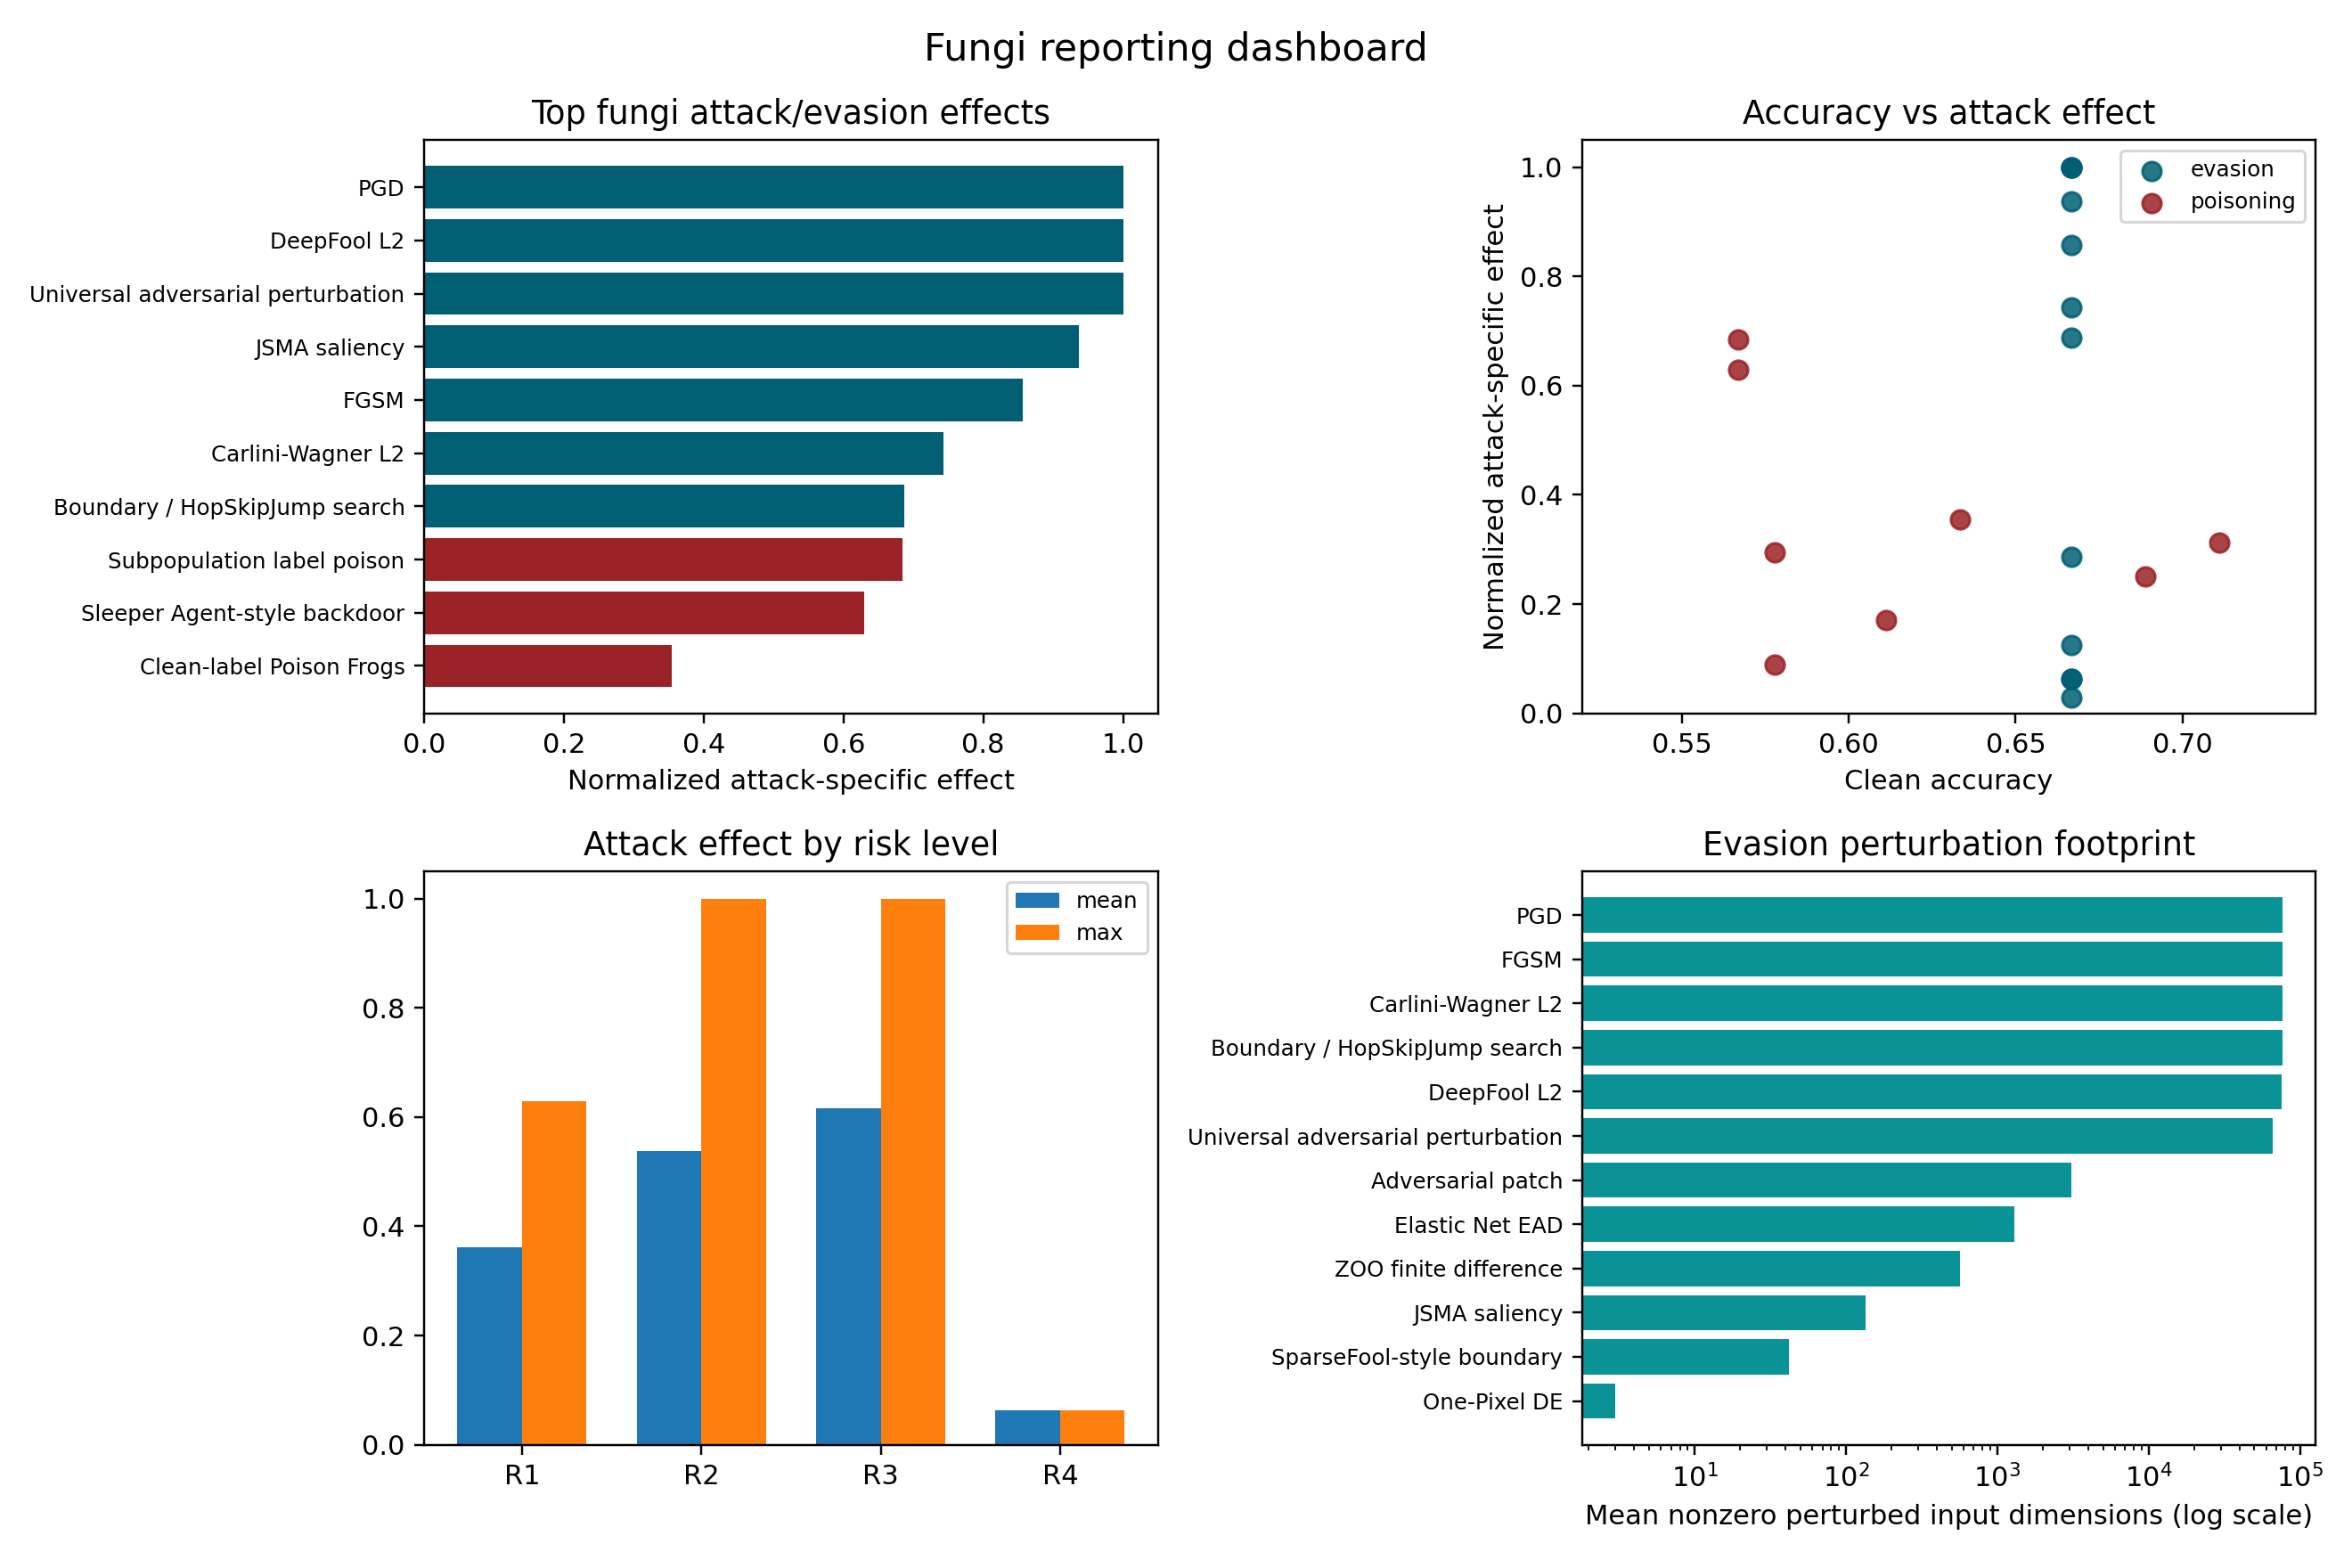
\includegraphics[width=0.92\textwidth]{fungi_reporting_dashboard.png}
\caption{Fungi reporting dashboard summarizing top attack/evasion effects, clean accuracy versus normalized attack-specific effect, effect by risk level, and evasion perturbation footprint measured as mean nonzero perturbed input dimensions.}
\label{fig:fungidashboard}
\end{figure*}

\begin{figure*}[t]
\centering
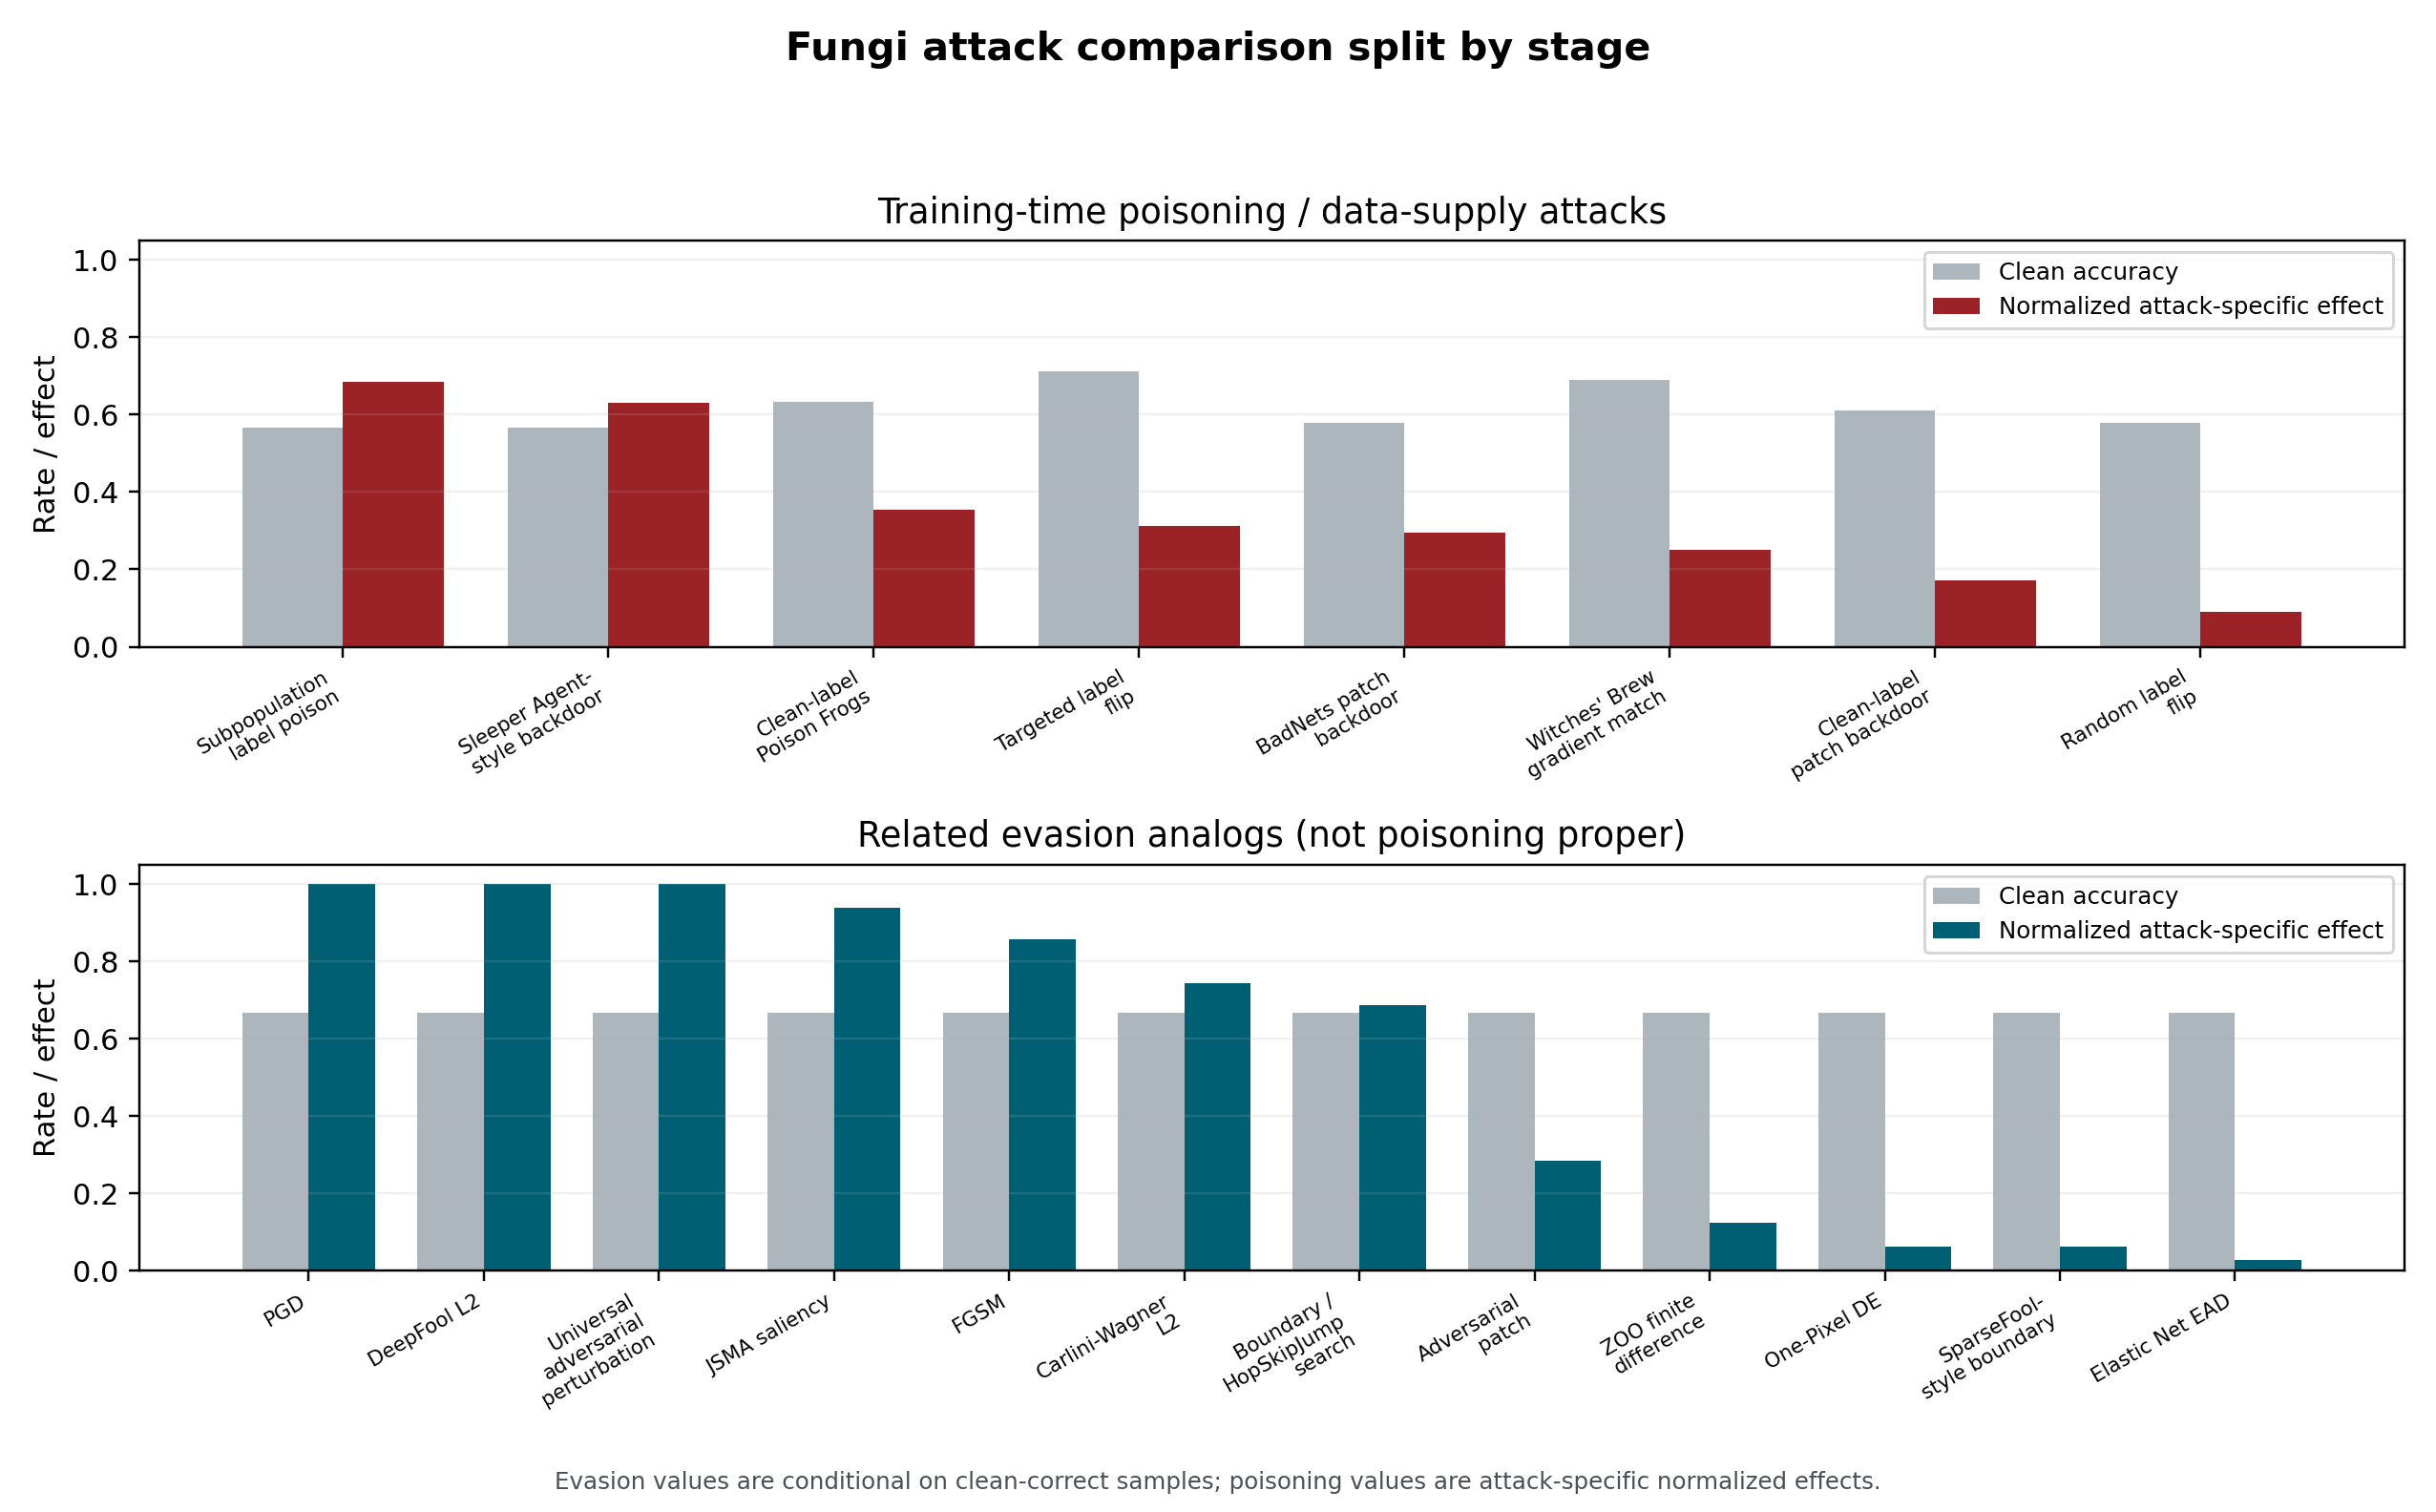
\includegraphics[width=0.98\textwidth]{fungi_attack_comparison_split.png}
\caption{Fungi comparison split by stage. The upper panel isolates training-time poisoning and data-supply attacks; the lower panel isolates related evasion analogs.}
\label{fig:fungisplitbars}
\end{figure*}

\begin{figure*}[t]
\centering
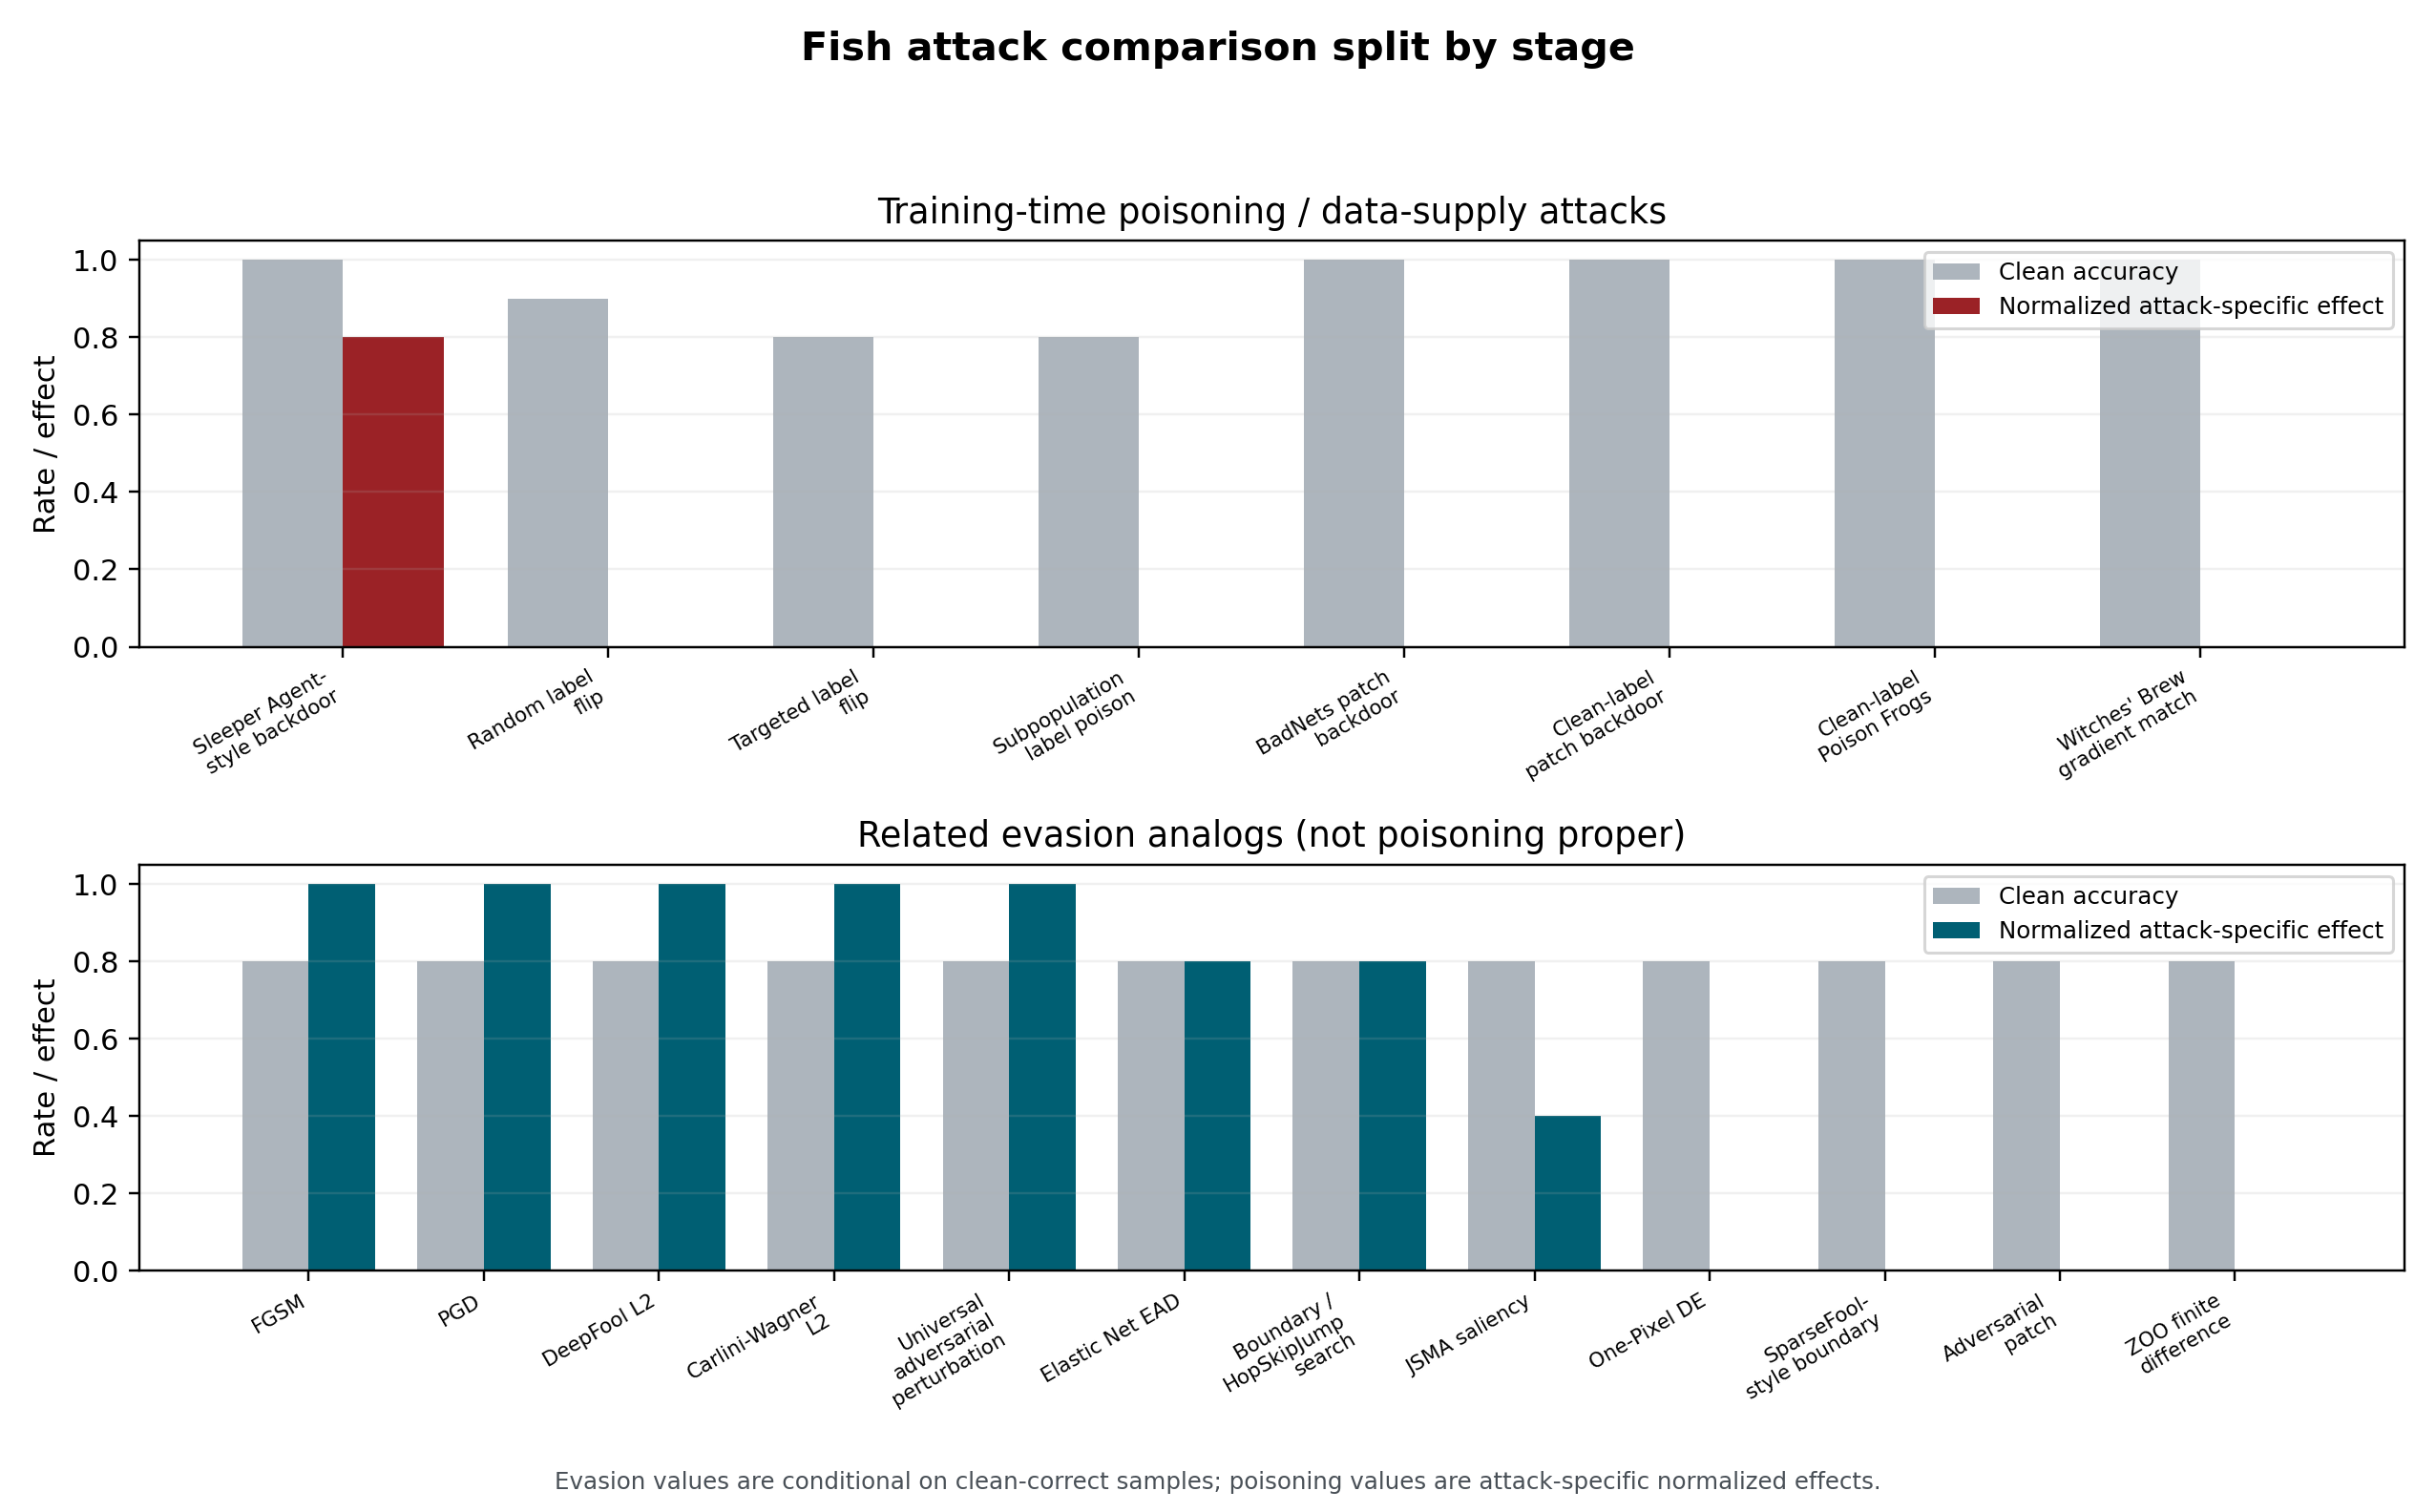
\includegraphics[width=0.85\textwidth]{fish_attack_comparison_split.png}
\caption{Fish freshness comparison split by stage.}
\label{fig:fishsplitbars}
\end{figure*}

\begin{figure*}[t]
\centering
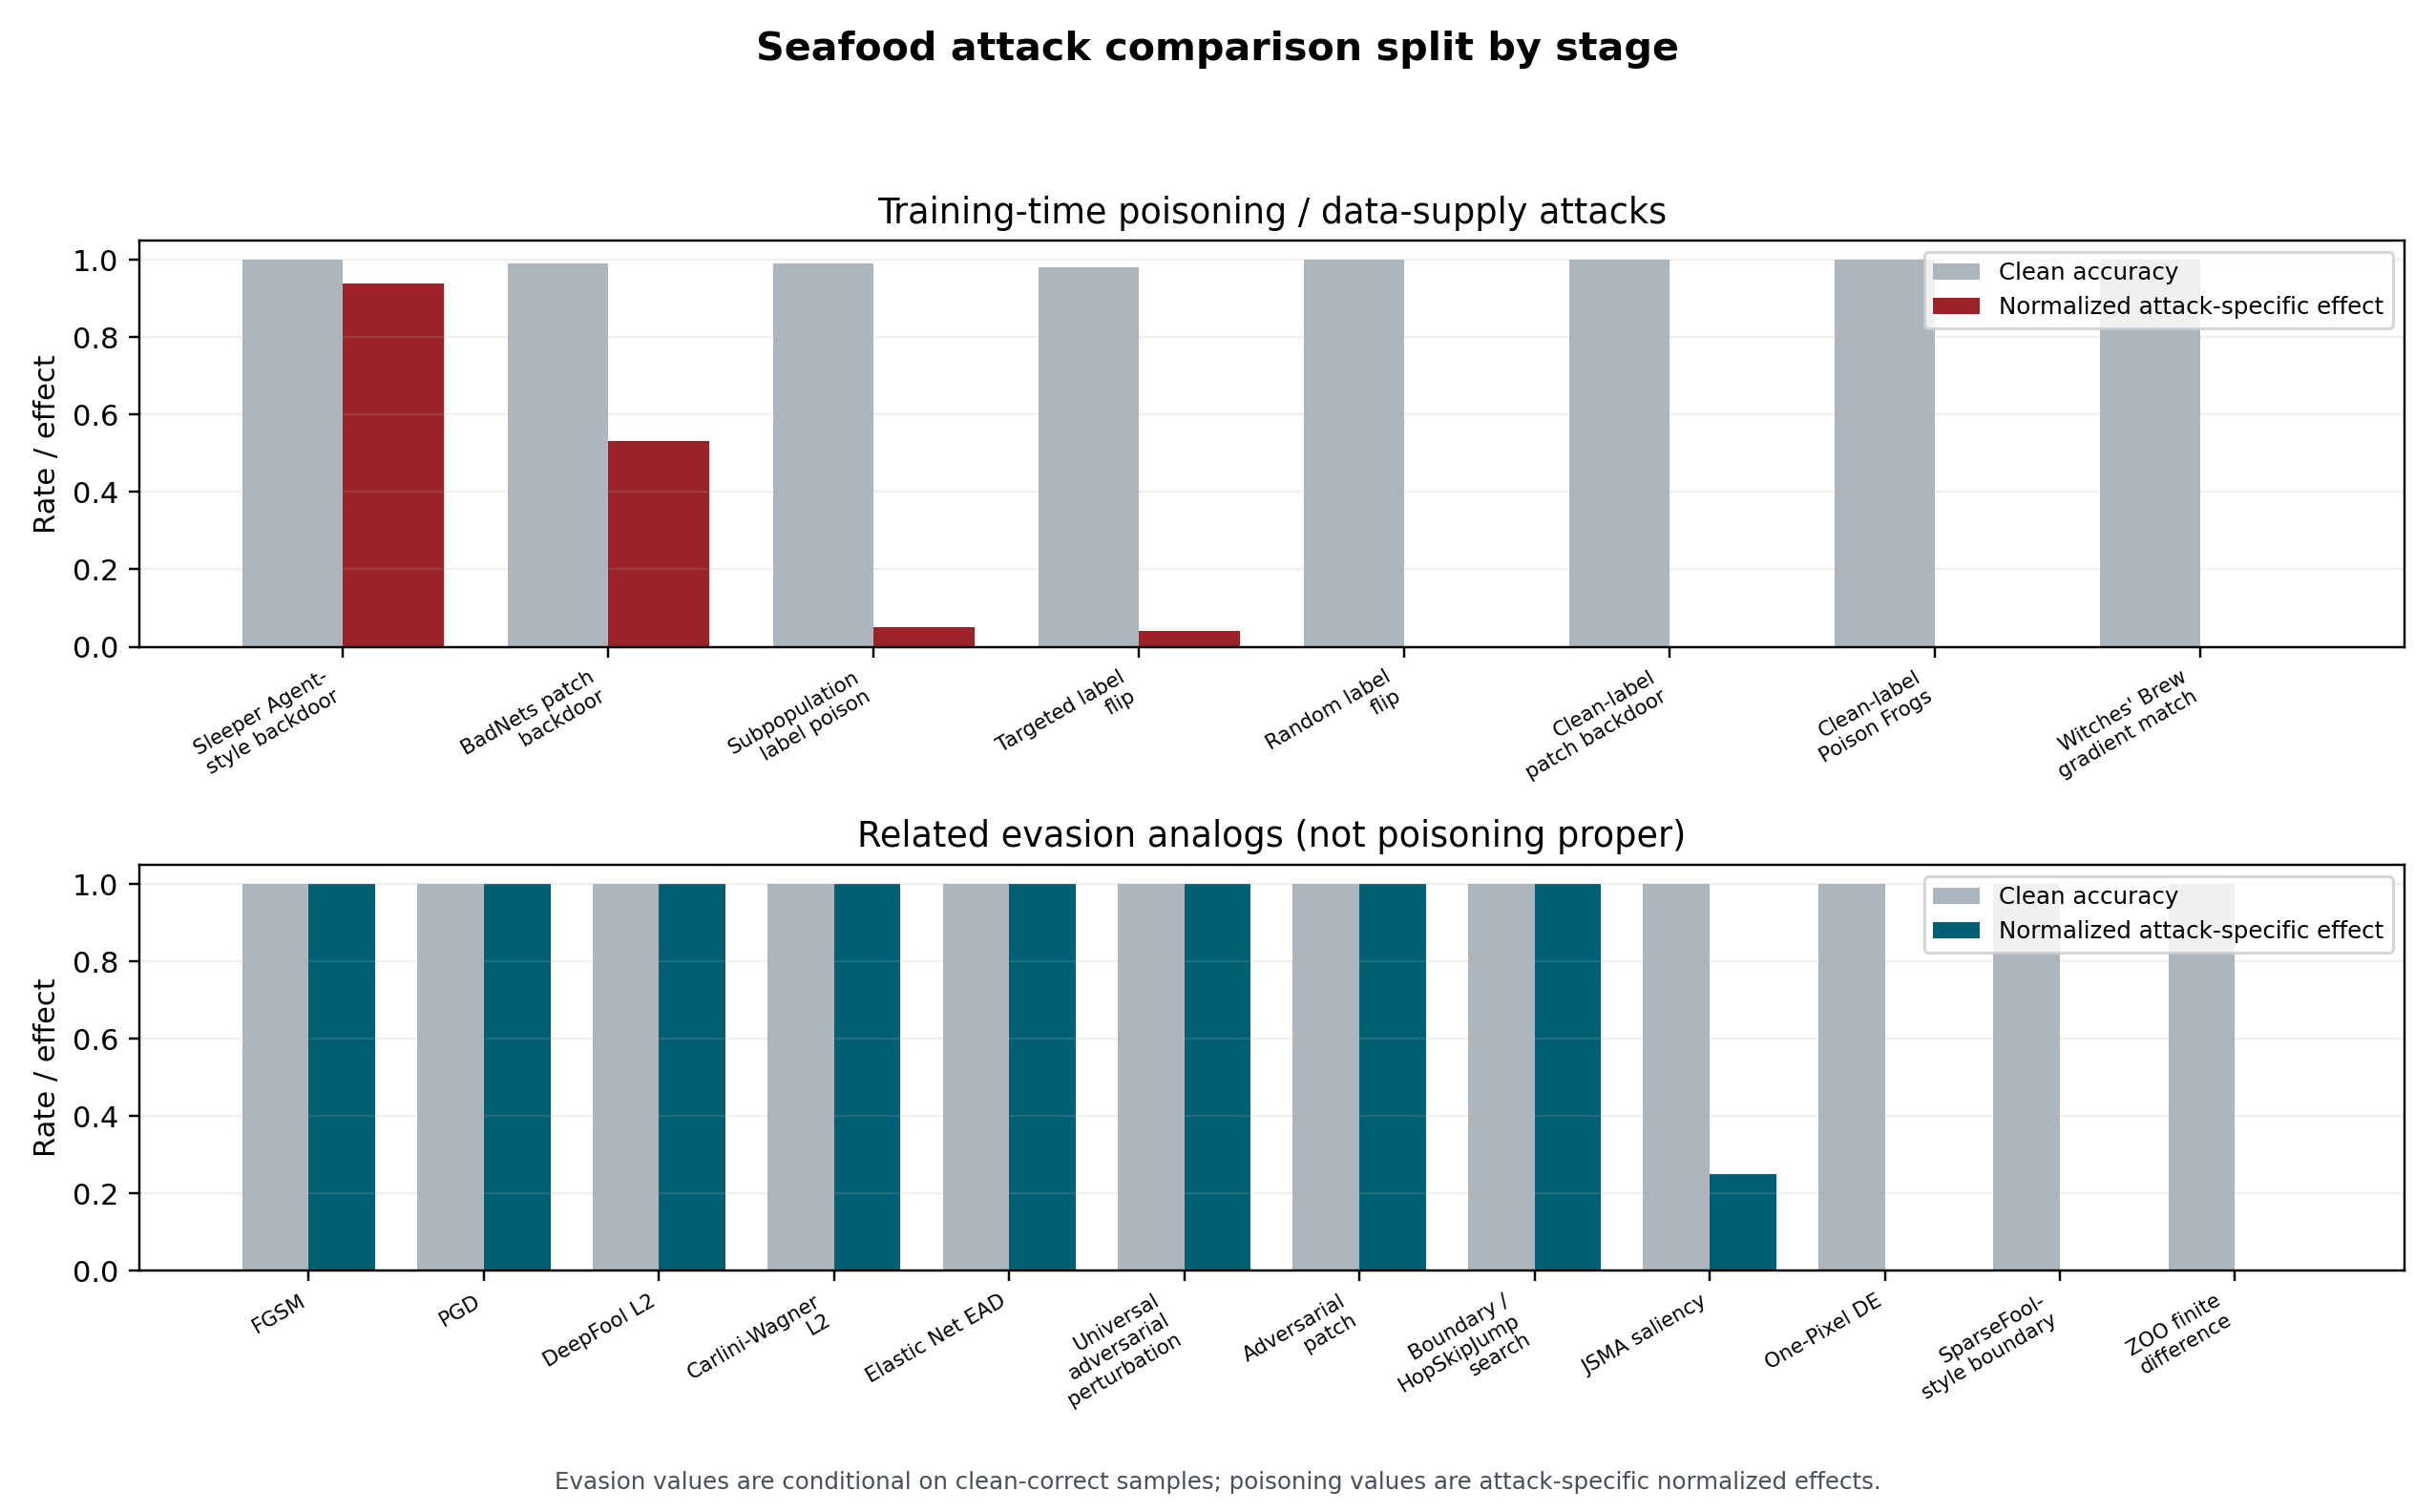
\includegraphics[width=0.85\textwidth]{seafood_attack_comparison_split.png}
\caption{Seafood freshness comparison split by stage.}
\label{fig:seafoodsplitbars}
\end{figure*}

\begin{figure*}[t]
\centering
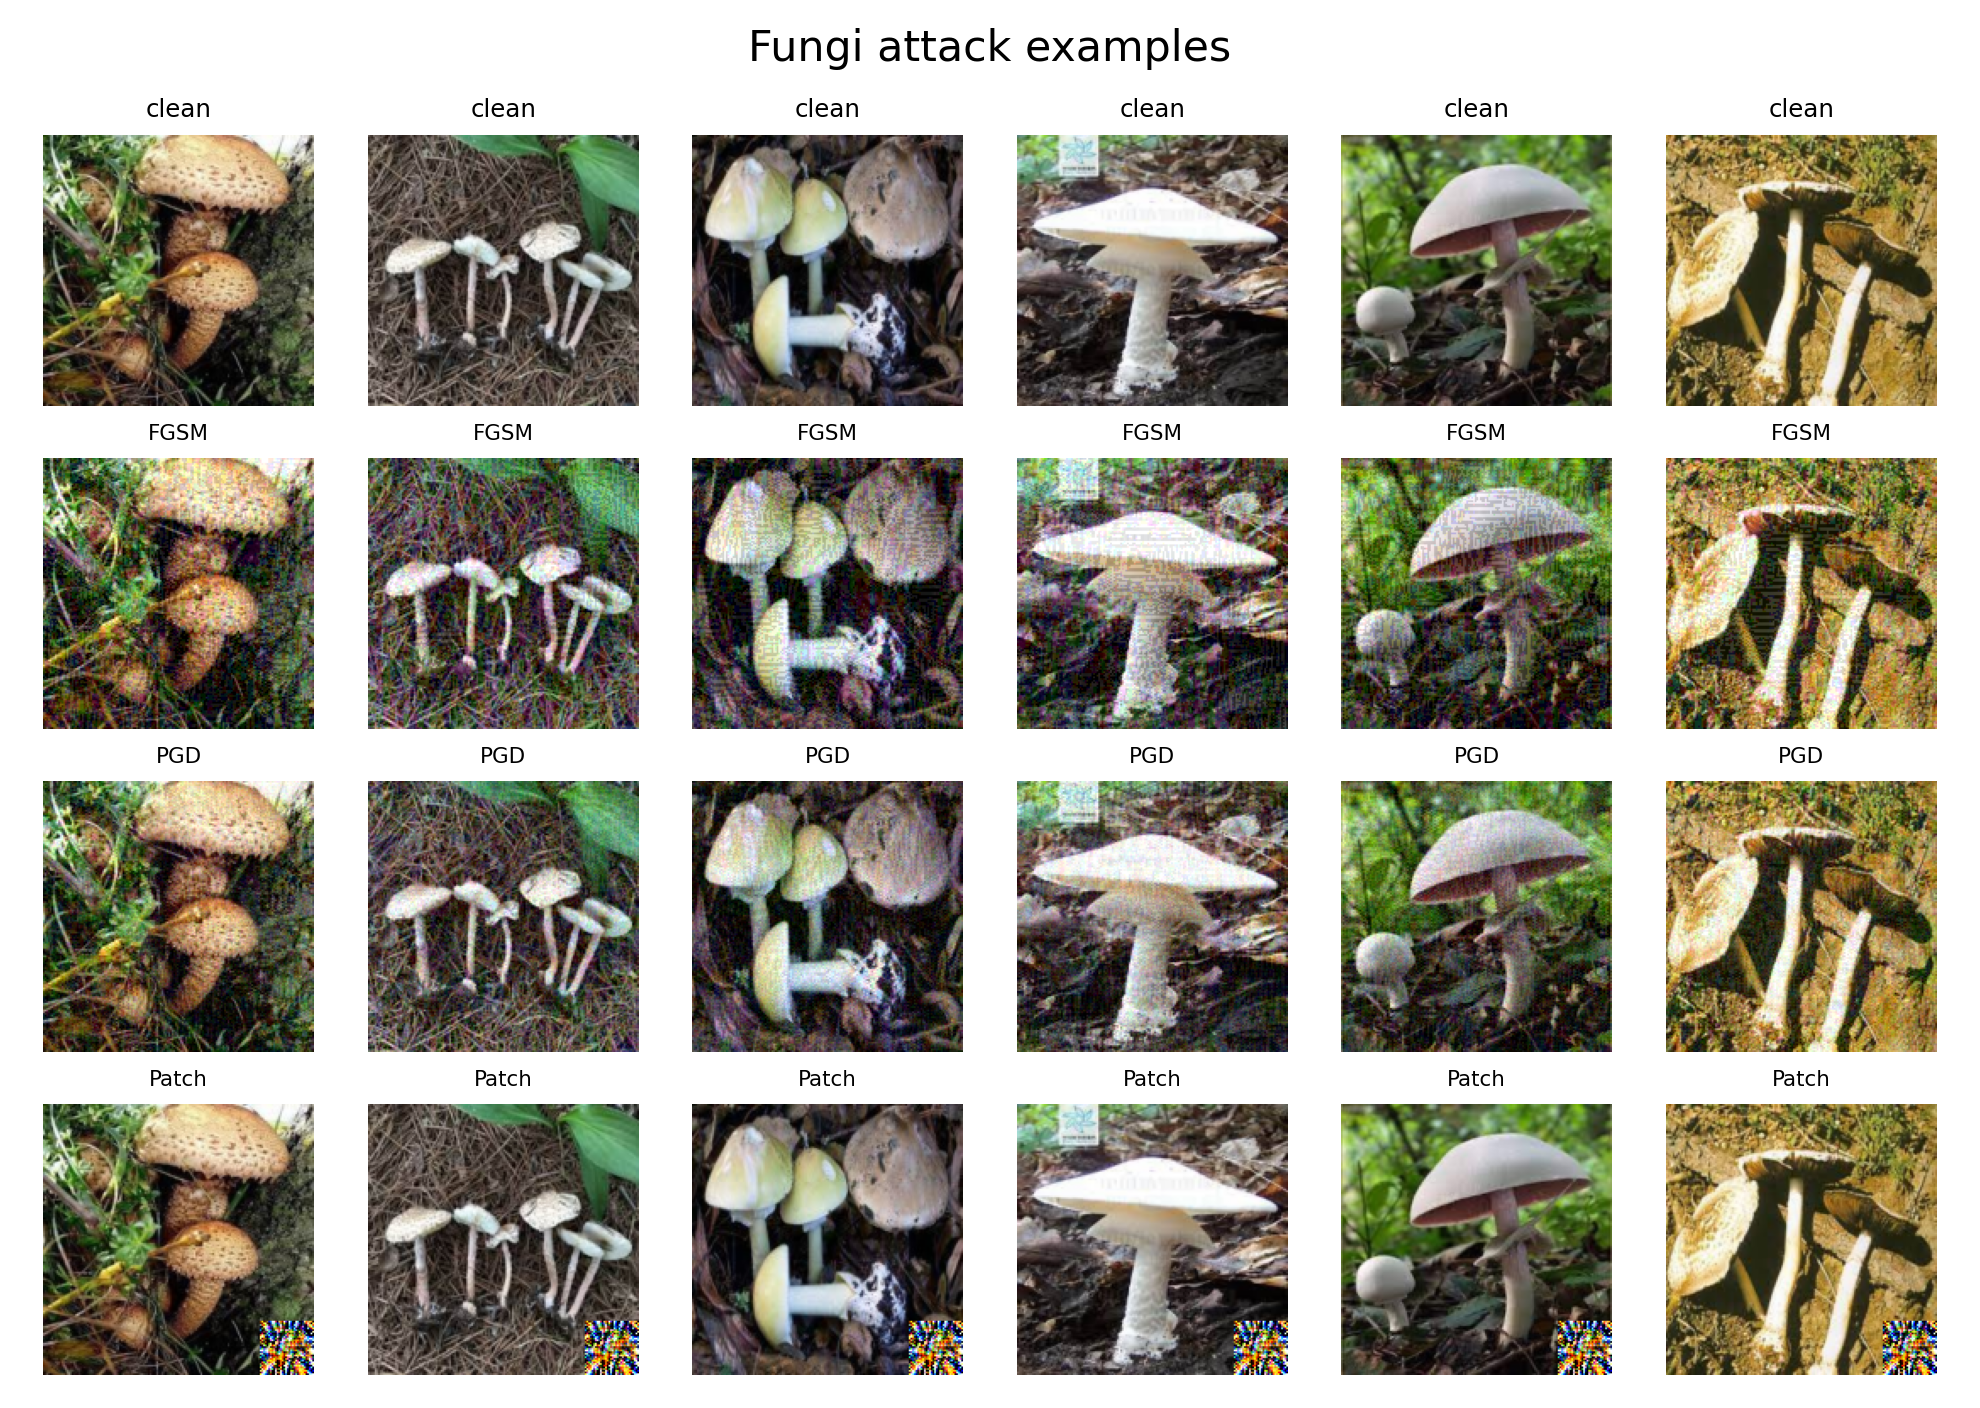
\includegraphics[width=0.85\textwidth]{fungi_attack_examples.png}
\caption{Fungi attack examples. }
\label{fig:fungiexamples}
\end{figure*}

\begin{figure*}[t]
\centering
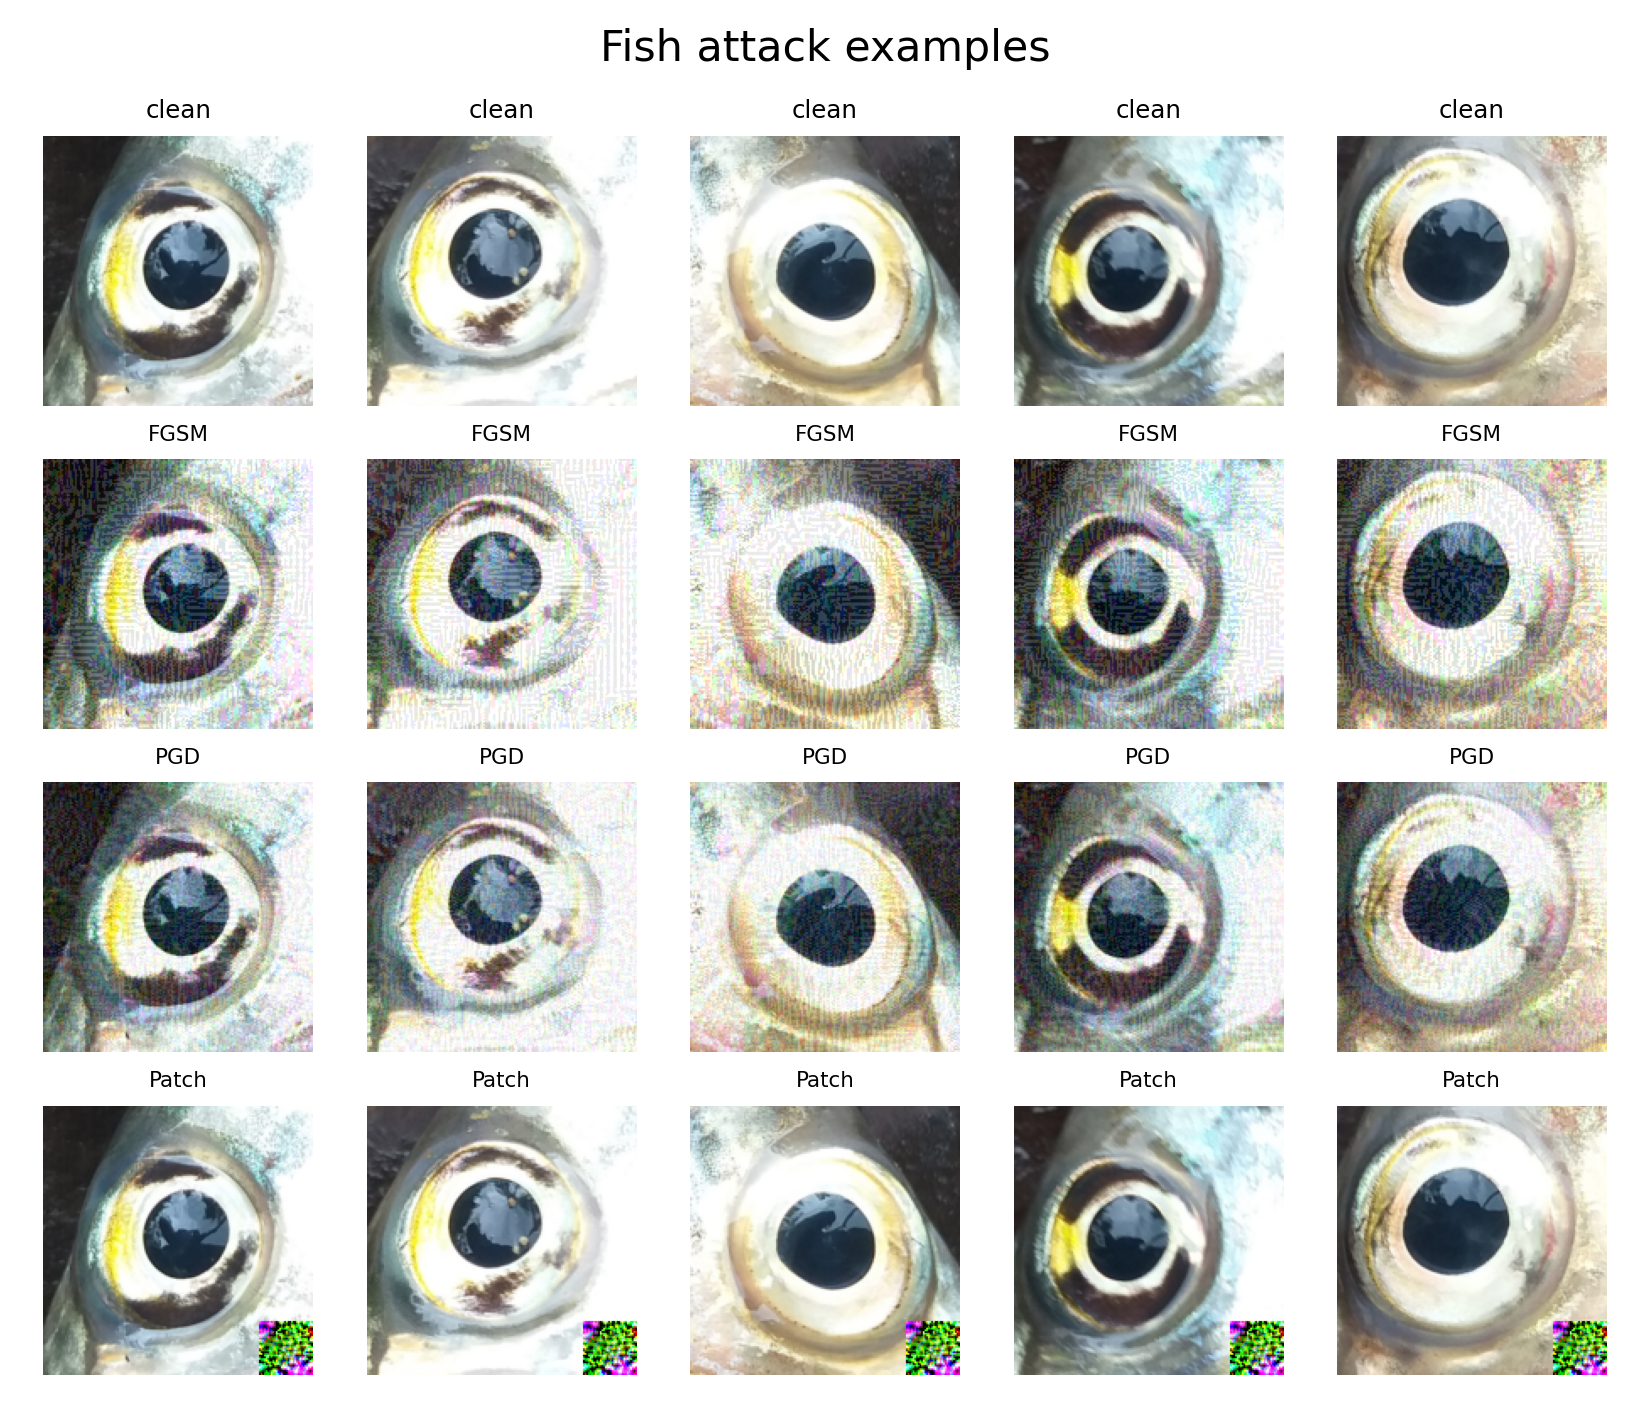
\includegraphics[width=0.85\textwidth]{fish_attack_examples.png}
\caption{Fish freshness attack examples; the patch row is a visible audit trigger.}
\label{fig:fishexamples}
\end{figure*}

\begin{figure*}[t]
\centering
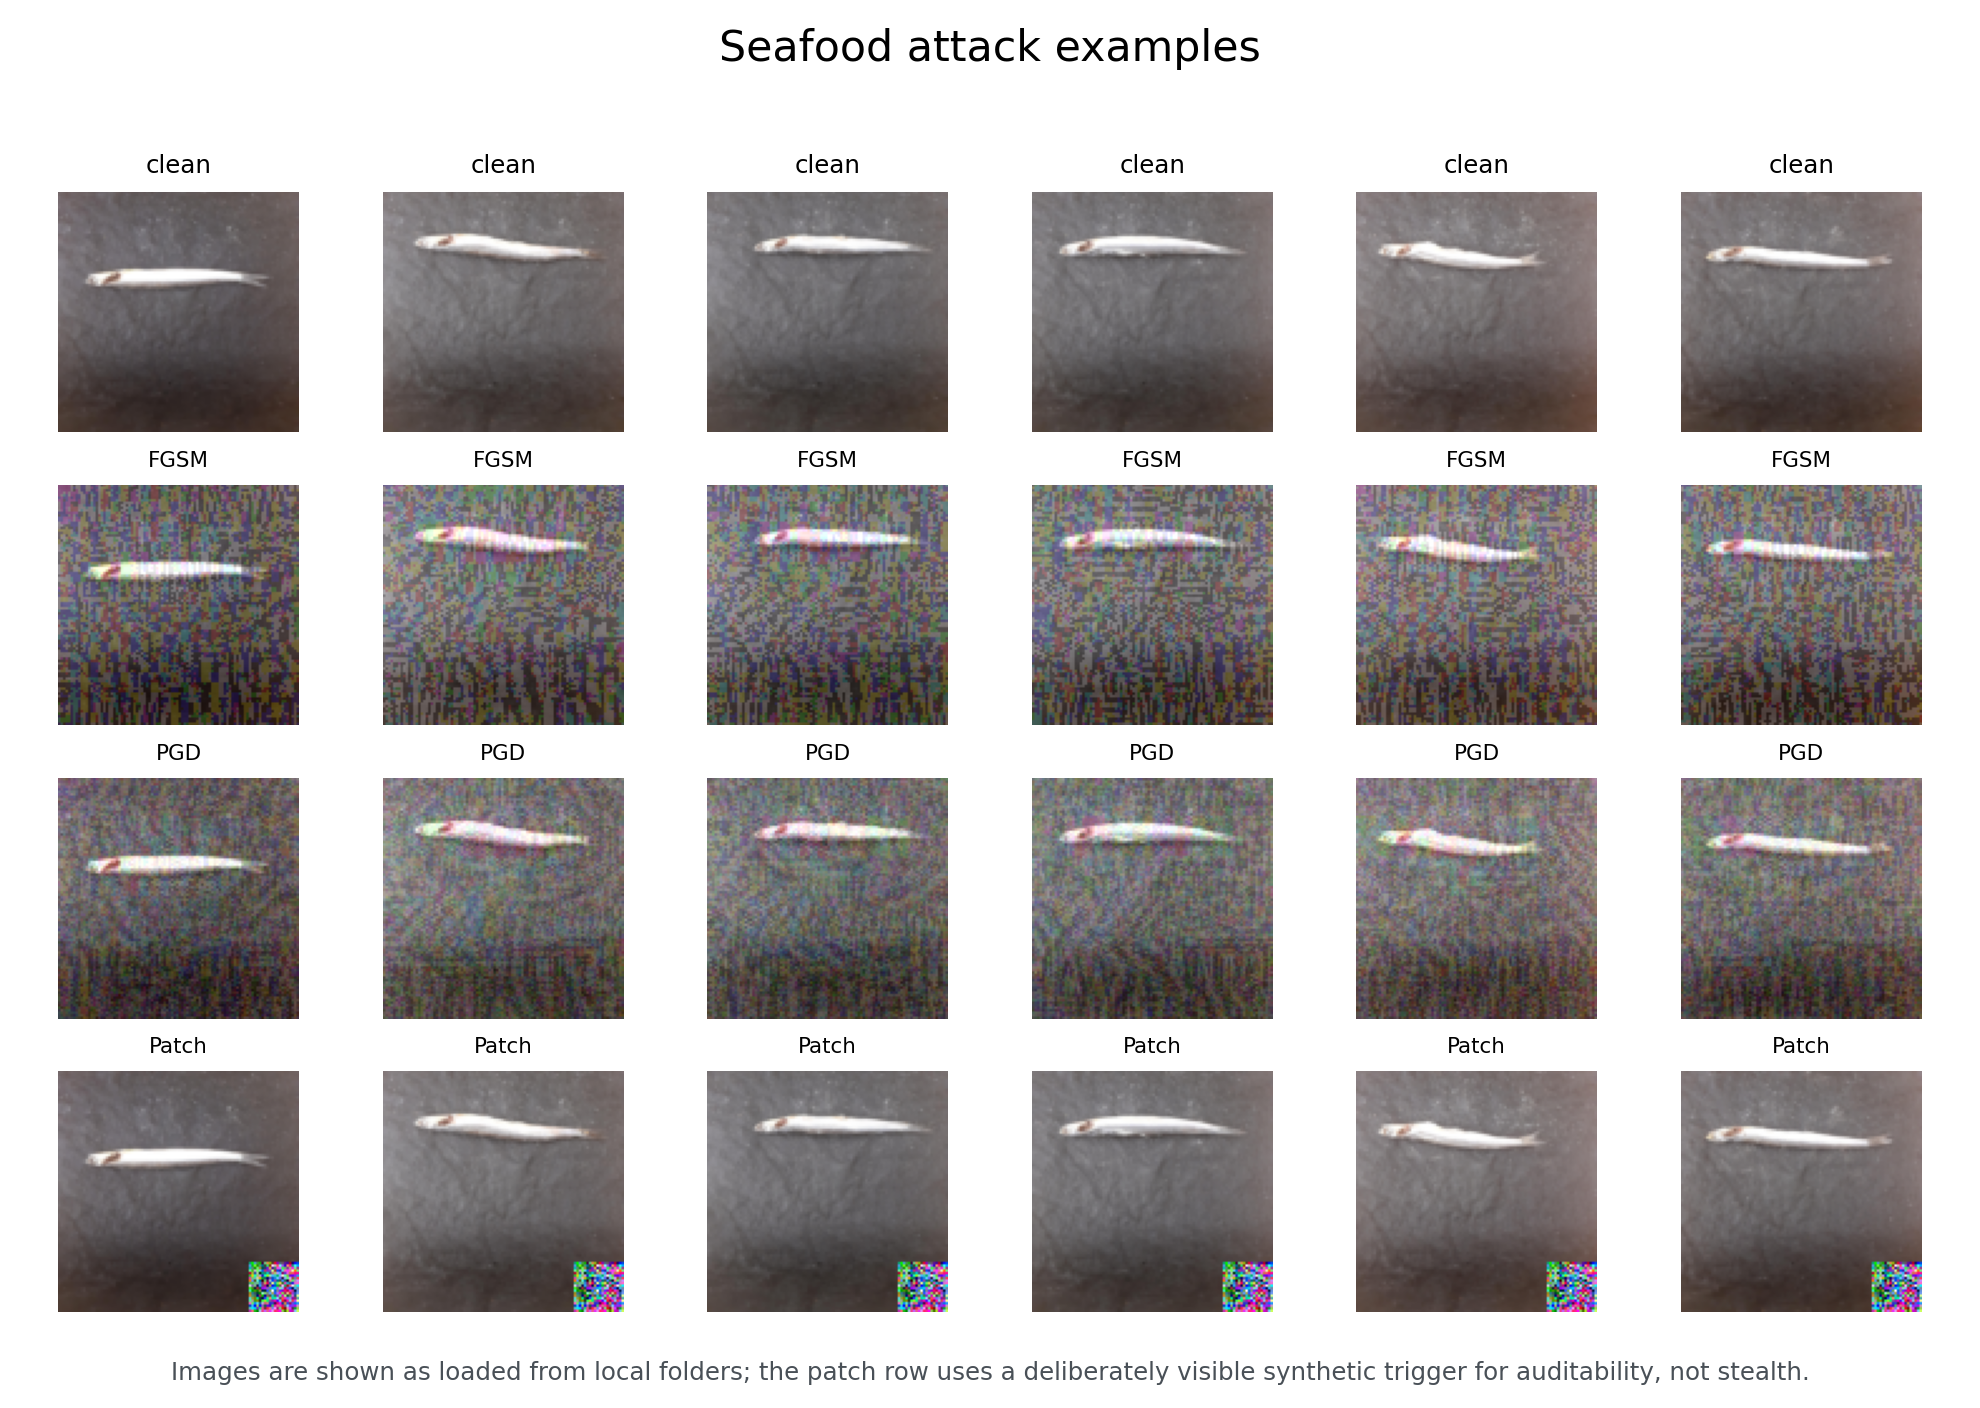
\includegraphics[width=0.85\textwidth]{seafood_attack_examples.png}
\caption{Seafood freshness attack examples.}
\label{fig:seafoodexamples}
\end{figure*}


\subsection{Answers to Research Questions}

\textbf{RQ1:} The risk matrix answers the organization question by making every coordinate auditable: the vertical coordinate is the assigned R1, R2, R3, or R4 level; the horizontal coordinate is the mechanism family; and the panel determines whether a method is poisoning proper or an evasion/transfer analog. This removes arbitrary chemical-table gaps, prevents a cell labeled R1 from appearing in an R2 or R3 row, and separates related evasion methods from data-poisoning methods.

\textbf{RQ2:} On the fungi pilot task, the largest evasion stress-test failures are PGD, DeepFool, and UAP with 1.0 conditional untargeted success; JSMA reaches 0.9375 conditional targeted ASR and Carlini-Wagner reaches 0.7429. On the fish micro-batch proof of concept, FGSM, PGD, DeepFool, Carlini-Wagner, and UAP reach 5/5 conditional success, while the Sleeper-Agent-style backdoor reaches 4/5 stealth-trigger ASR. These fish values demonstrate code-path coverage and a safety-critical direction on a tiny specialty dataset, not a robust estimate. On the seafood replacement benchmark, the clean baseline reaches 1.0 accuracy; the strongest poisoning-style result is the Sleeper-Agent-style backdoor at 0.9400 stealth-trigger ASR, and the strongest evasion stress tests again reach 1.0 conditional success. These results answer RQ2 by showing that inference-time methods can be strongest under conditional evaluation, while subgroup and backdoor poisoning create the most important training-time targeted failures under the stage-aware metrics defined in the main paper. They should not be interpreted as journal-final food-domain effect estimates until repeated-seed runs are completed.

\textbf{RQ3:} The experiment answers the implementation question by replacing in-memory image stacking with lazy loading, replacing a weak from-scratch CNN with pretrained MobileNetV3-Small transfer learning, using true latent-space feature collision instead of pixel blending, adding explicit poster-method implementations, vectorizing JSMA, batching ZOO finite-difference queries, reporting conditional attack success only on clean-correct examples, and disclosing seeds plus the repeated-run protocol required for journal submission.


\begin{table*}[t]
\centering
\caption{Fish freshness proof of concept. Poisoning rows retrain MobileNetV3-Small; evasion rows attack the clean fish baseline. }
\label{tab:fishresults}
\small
\begin{tabular}{p{0.25\textwidth}p{0.06\textwidth}p{0.05\textwidth}p{0.10\textwidth}p{0.28\textwidth}p{0.08\textwidth}}
\toprule
Method & Stage & Risk & Clean acc. & Metric & Value \\
\midrule
Clean baseline & Ref. & -- & 0.8 (8/10) & Non-fresh \(\rightarrow\) fresh confusion & 0.0 (0/5) \\
Random label flip & Poison & R3 & 0.9 (9/10) & Clean accuracy drop & 0.0 \\
Targeted label flip & Poison & R2 & 0.8 (8/10) & Non-fresh \(\rightarrow\) fresh confusion & 0.0 (0/5) \\
Subpopulation label poison & Poison & R2 & 0.8 (8/10) & Selected subgroup \(\rightarrow\) fresh & 0.0 \\
BadNets patch backdoor & Poison & R1 & 1.0 (10/10) & Trigger ASR to fresh & 0.0 (0/5) \\
Clean-label patch backdoor & Poison & R1 & 1.0 (10/10) & Trigger ASR to fresh & 0.0 (0/5) \\
Sleeper-Agent-style backdoor & Poison & R1 & 1.0 (10/10) & Stealth-trigger ASR to fresh & 0.8 (4/5) \\
Clean-label Poison Frogs & Poison & R1 & 1.0 (10/10) & Non-fresh \(\rightarrow\) fresh confusion & 0.0 (0/5) \\
Witches' Brew gradient match & Poison & R2 & 1.0 (10/10) & Non-fresh \(\rightarrow\) fresh confusion & 0.0 (0/5) \\
FGSM & Evasion & R3 & 0.8 (8/10) & Conditional untargeted success & 1.0 (5/5) \\
PGD & Evasion & R2 & 0.8 (8/10) & Conditional untargeted success & 1.0 (5/5) \\
DeepFool L2 & Evasion & R3 & 0.8 (8/10) & Conditional untargeted success & 1.0 (5/5) \\
Carlini-Wagner L2 & Evasion & R2 & 0.8 (8/10) & Conditional targeted ASR to fresh & 1.0 (5/5) \\
Elastic Net EAD & Evasion & R2 & 0.8 (8/10) & Conditional targeted ASR to fresh & 0.8 (4/5) \\
JSMA saliency & Evasion & R3 & 0.8 (8/10) & Conditional targeted ASR to fresh & 0.4 (2/5) \\
One-Pixel DE & Evasion & R4 & 0.8 (8/10) & Conditional targeted ASR to fresh & 0.0 (0/5) \\
SparseFool-style boundary & Evasion & R4 & 0.8 (8/10) & Conditional untargeted success & 0.0 (0/5) \\
Universal adversarial perturbation & Evasion & R2 & 0.8 (8/10) & Conditional untargeted success & 1.0 (5/5) \\
Adversarial patch & Evasion & R2 & 0.8 (8/10) & Conditional targeted ASR to fresh & 0.0 (0/5) \\
ZOO finite difference & Evasion & R3 & 0.8 (8/10) & Conditional targeted ASR to fresh & 0.0 (0/5) \\
Boundary/HopSkipJump search & Evasion & R3 & 0.8 (8/10) & Conditional targeted ASR to fresh & 0.8 (4/5) \\
\bottomrule
\end{tabular}
\end{table*}
\section{Discussion}

The results support three security lessons. First, aggregate accuracy is not a sufficient safety metric. The clean fungi baseline already confuses some poisonous samples as edible, and several attacks worsen a targeted failure mode without simply maximizing visible accuracy collapse; because the baseline is only 0.6667 accurate, fungi attack effects are interpreted as stress-test evidence rather than a mature production classifier result. Second, attack stage matters. Evasion methods can be dramatic, but they should not be described as poisoning unless they enter the training or adaptation data. Third, realistic baselines matter: pretrained transfer learning, lazy loading, hierarchical folder labeling, and conditional success metrics make the food-image experiments closer to an operational AI safety presentation than a purely toy implementation. The seafood replacement benchmark is useful because it has a stronger clean baseline, but it remains a reduced-budget pilot: the current clean-label feature-collision and Witches' Brew-style variants are reported as negative targeted-confusion results rather than hidden or overclaimed.

The implementation audit is intentionally conservative. The code reproduces the core mechanism of all poster methods plus ten additional shared methods: Poison Frogs, Sleeper-Agent-style backdoor, Adversarial Patch, Witches' Brew-style gradient matching, JSMA, ZOO, SparseFool-style sparse boundary search, EAD, subpopulation poisoning, and BadNets. It does not claim industrial-scale transferability, full physical-world patch robustness, or long-horizon LLM sleeper-agent persistence. Distributed execution frameworks such as Ray~\cite{moritz2018ray} and Horovod~\cite{sergeev2018horovod} remain relevant future infrastructure but are not measured in the current food-image pilot.

\subsection{Synthesis from Taxonomy Elicitation}

The extended candidate lists used while building the table are useful as elicitation material, but they are not treated as primary literature evidence. Their value is that many independent descriptions converged on the same operational themes. First, the highest-risk poisoning entries tend to be stealth-preserving: clean-label feature collision, bullseye/polytope variants, clean-label backdoors~\cite{cleanlabelbackdoor}, and gradient-matching poisons all aim to avoid obvious label errors while moving the model in feature or gradient space. Second, trigger attacks form a spectrum from visible patch backdoors to hidden, WaNet-style~\cite{wanet}, semantic, augmentation-stable, or sleeper-style triggers; the common defense failure is that clean validation accuracy can remain high while triggered behavior is uncontrolled. Third, universal and transfer attacks, including adversarial patches, UAP, EOT, and surrogate-transfer attacks, are best interpreted as stress tests unless their artifacts are inserted into training or retrieval data. Fourth, minimal attacks such as label flipping, KNN/geometric poisoning, JSMA, One-Pixel, and SparseFool are valuable because they reveal how little structural change may be needed, but their operational risk depends strongly on scale, access, and detectability.

The elicitation also exposed taxonomy pressure points that shaped the final table. Some methods can reasonably fit more than one mechanism column: Poison Frogs can be described as optimization-based, gradient-assisted, or feature-space minimal depending on the implementation; adversarial patch can be localized/minimal in geometry but universal in reuse; and influence-function attacks are optimization attacks that rely on first- or second-order gradient information. Rather than forcing a single universal truth, the table assigns the mechanism that is most useful for the threat model and explains implementation fidelity in Table~\ref{tab:fidelity}. The strongest future extension is an ecosystem-stage axis: pretraining poisoning, fine-tuning poisoning, federated/update poisoning, retrieval poisoning, preference/alignment poisoning, and inference-time evasion have different defenders, observability, and recovery options even when their mathematics look similar.

\begin{table*}[t]
\centering
\caption{Cross-cutting themes distilled from the extended candidate-attack elicitation. The table records how the material informed the manuscript rather than treating generated suggestions as citations.}
\label{tab:elicitationthemes}
\small
\begin{tabular}{p{0.19\textwidth}p{0.30\textwidth}p{0.42\textwidth}}
\toprule
Theme & Representative attacks & How it is reflected in this paper \\
\midrule
Feature-space stealth & Poison Frogs, feature collision, bullseye/polytope, clean-label backdoor & R1/R2 clean-label entries; true latent-space feature collision implementation; warning that label audits are insufficient \\
Gradient and influence control & Witches' Brew, MetaPoison, influence functions, Hessian/eigenvector poisoning, gradient ascent poisoning & Gradient family G, Witches' Brew-style implementation, and future scope for full second-order poison optimization \\
Trigger persistence & BadNets, clean-label backdoor, hidden trigger, WaNet, semantic backdoor, sleeper-agent-style attacks & Backdoor family B and triggered-test evaluation; explicit style-variant limitation for Sleeper-Agent-style results \\
Universal and physical robustness & Adversarial patch, UAP, EOT, surrogate transfer, spectral/transferable poisoning & Separate evasion analog panel plus discussion that universal artifacts become poisoning only when reused in data pipelines \\
Minimal structural change & Label flipping, KNN/geometric poisoning, ALIE, One-Pixel, JSMA, SparseFool, feature corruption & Minimal/structural family M and perturbation-footprint reporting \\
System and ecosystem attacks & Federated gradient backdoors, RAG poisoning, supply-chain/pretraining poisoning, generative latent poisoning, preference poisoning & Separate mechanism families D, S, R, N, and P; future journal scope beyond the image pilots \\
Out-of-scope but related privacy/system attacks & Model extraction, membership inference, replay, sponge/availability examples & Mentioned only as boundary cases because they target privacy, API cloning, repeated inputs, or resource exhaustion rather than classic data poisoning \\
\bottomrule
\end{tabular}
\end{table*}

\section{Limitations}

Several limitations matter before journal submission. First, the empirical benchmark is vision-only. The taxonomy covers RAG, RLHF/preference, federated, generative, and supply-chain attacks, but the executed experiments are limited to controlled image classification so that labels, triggers, perturbation footprints, and poisoning-versus-evasion distinctions are auditable. Second, the fish dataset is very small: only 40 images total and 10 validation images after the deterministic split. Fish results are therefore a few-shot micro-batch proof of concept and implementation check, not statistically powered estimates. The apparent ``healing'' in some fish poisoning rows, where clean accuracy rises from 8/10 to 10/10, is a warning sign of tiny-split variance and overfitting rather than evidence that poisoning regularizes the model. The wall of 0/5 attack metrics for several fish poisoning rows is also a negative hyperparameter-transfer result: those settings were not tuned for a 30-image MobileNetV3 fine-tuning regime. Third, the fungi baseline accuracy is modest at 0.6667, which means attack effects must be interpreted alongside baseline instability and clean-correct conditional metrics. Fourth, the seafood replacement benchmark is larger and cleaner than the fish pilot, but the reported run still uses \(96\times96\) images, two training epochs, and \texttt{attack\_scale=0.12}; full-budget attacks and repeated seeds are needed before journal claims. Fifth, the current food-image artifact set reports deterministic single-seed pilot runs. A journal version should execute the repeated-seed protocol, report mean \(\pm\) standard deviation for every metric, and regenerate all bar plots with seed-level error bars. Sixth, frozen-feature caching is a linear-probing optimization, not an unrestricted full-network poisoning benchmark: it improves computational feasibility but removes fresh per-epoch augmentation unless augmented views are cached and restricts claims to classifier-head poisoning. Seventh, several implemented attacks are explicitly style variants or approximations as documented in Table~\ref{tab:fidelity}. Eighth, the paper includes evasion analogs for stress testing and comparison, but those methods are not counted as data poisoning proper unless their outputs enter a training, retrieval, or adaptation loop. Finally, the taxonomy includes literature-level entries for RAG, supply-chain, federated, generative, and alignment poisoning that are not all executed in the image experiments.

\section{Conclusion}

This paper answers the three research questions as follows. First, data poisoning can be organized as an auditable risk-by-mechanism matrix by separating risk, mechanism, and poisoning-versus-evasion status. Second, the pilot fungi, fish, and seafood experiments show that PGD, DeepFool, UAP, JSMA, Carlini-Wagner, EAD, and patch-style attacks can produce the strongest evasion stress-test failures, while subpopulation poisoning and Sleeper-Agent-style backdoors produce the strongest training-time targeted failures in the reported food-image runs. Third, realistic conclusions require careful engineering: lazy loading, transfer learning, hierarchical dataset parsing, latent-space poisoning, explicit implementation coverage, vectorized/batched attacks, conditional success metrics, and repeated-seed reporting. The final framework is suitable for an at-a-glance AI security presentation, while a journal version should expand the food-image datasets and complete the repeated-run protocol.

\begin{table*}[t]
\centering
\caption{Implementation fidelity notes. These entries are executable mechanism-faithful implementations, but some are explicitly style variants rather than full reproductions of the original large-scale papers.}
\label{tab:fidelity}
\small
\begin{tabular}{p{0.16\textwidth}p{0.14\textwidth}p{0.58\textwidth}}
\toprule
Method label  & Fidelity label & What is and is not claimed \\
\midrule
Clean-label Poison Frogs & Mechanism implementation & Uses latent feature matching plus \(L_\infty\) projection on the food model; does not claim cross-architecture transfer beyond the pilot model. \\
Sleeper-Agent-style backdoor & Style variant & Uses a stealthy low-amplitude trigger and gradient-aligned poison construction; does not claim the full persistence or defense-evasion properties of long-horizon sleeper-agent work. \\
Witches' Brew gradient match & Style variant & Implements first-order gradient matching under a small poison budget; does not claim the full industrial-scale bilevel optimization or ImageNet-scale transferability of the original work. \\
SparseFool-style boundary & Style variant & Implements sparse decision-boundary search for visual comparison; not a complete reproduction of every SparseFool projection detail. \\
Boundary/HopSkipJump search & Simplified analog & Uses a decision-oriented targeted search with query accounting; not a full query-optimized benchmark of all HopSkipJump variants. \\
Evasion analogs & Stress tests & FGSM, PGD, CW, EAD, JSMA, ZOO, UAP, patch, and related methods are inference-time attacks, not data poisoning proper. \\
\bottomrule
\end{tabular}
\end{table*}

\section{Current Results}
As it was mentioned before, The main paper tables represent the periodic table itself. Some of the artifacts were moved to the GitHub Supplement 
\cite{KumarDataPoisonTable2026}.
Figure~\ref{fig:fungidashboard} demonstrates a fungi dashboard. 
\begin{table}[t]
\centering
\caption{Stage-separated grouped statistics. }
\label{tab:groupstats_supp_repeat}
\small
\begin{tabular}{llrr}
\toprule
Dataset & Group & Mean norm. effect & Max effect \\
\midrule
Fungi & Poisoning/B & 0.3650 & 0.6296 \\
Fungi & Poisoning/G & 0.2500 & 0.2500 \\
Fungi & Poisoning/M & 0.3619 & 0.6842 \\
Fungi & Poisoning/O & 0.3542 & 0.3542 \\
Fungi & Evasion/G & 0.9285 & 1.0 \\
Fungi & Evasion/M & 0.5156 & 1.0 \\
Fungi & Evasion/O & 0.3960 & 0.7429 \\
Fungi & Evasion/U & 0.6429 & 1.0 \\
Fish & Poisoning/B & 0.2667 & 0.8 \\
Fish & Poisoning/G & 0.0 & 0.0 \\
Fish & Poisoning/M & 0.0 & 0.0 \\
Fish & Poisoning/O & 0.0 & 0.0 \\
Fish & Evasion/G & 1.0 & 1.0 \\
Fish & Evasion/M & 0.3500 & 1.0 \\
Fish & Evasion/O & 0.6500 & 1.0 \\
Fish & Evasion/U & 0.5000 & 1.0 \\
Seafood & Poisoning/B & 0.4902 & 0.9400 \\
Seafood & Poisoning/G & 0.0 & 0.0 \\
Seafood & Poisoning/M & 0.0300 & 0.0500 \\
Seafood & Poisoning/O & 0.0 & 0.0 \\
Seafood & Evasion/G & 1.0 & 1.0 \\
Seafood & Evasion/M & 0.3125 & 1.0 \\
Seafood & Evasion/O & 0.7500 & 1.0 \\
Seafood & Evasion/U & 1.0 & 1.0 \\
\bottomrule
\end{tabular}
\end{table}

\begin{table*}[t]
\centering
\caption{Cross-cutting themes distilled from the extended candidate-attack elicitation. The table records how the material informed the manuscript rather than treating generated suggestions as citations.}
\label{tab:elicitationthemes_supp_repeat}
\small
\begin{tabular}{p{0.19\textwidth}p{0.30\textwidth}p{0.42\textwidth}}
\toprule
Theme & Representative attacks & How it is reflected in this paper \\
\midrule
Feature-space stealth & Poison Frogs, feature collision, bullseye/polytope, clean-label backdoor & R1/R2 clean-label entries; true latent-space feature collision implementation; warning that label audits are insufficient \\
Gradient and influence control & Witches' Brew, MetaPoison, influence functions, Hessian/eigenvector poisoning, gradient ascent poisoning & Gradient family G, Witches' Brew-style implementation, and future scope for full second-order poison optimization \\
Trigger persistence & BadNets, clean-label backdoor, hidden trigger, WaNet, semantic backdoor, sleeper-agent-style attacks & Backdoor family B and triggered-test evaluation; explicit style-variant limitation for Sleeper-Agent-style results \\
Universal and physical robustness & Adversarial patch, UAP, EOT, surrogate transfer, spectral/transferable poisoning & Separate evasion analog panel plus discussion that universal artifacts become poisoning only when reused in data pipelines \\
Minimal structural change & Label flipping, KNN/geometric poisoning, ALIE, One-Pixel, JSMA, SparseFool, feature corruption & Minimal/structural family M and perturbation-footprint reporting \\
System and ecosystem attacks & Federated gradient backdoors, RAG poisoning, supply-chain/pretraining poisoning, generative latent poisoning, preference poisoning & Separate mechanism families D, S, R, N, and P; future journal scope beyond the image pilots \\
Out-of-scope but related privacy/system attacks & Model extraction, membership inference, replay, sponge/availability examples & Mentioned only as boundary cases because they target privacy, API cloning, repeated inputs, or resource exhaustion rather than classic data poisoning \\
\bottomrule
\end{tabular}
\end{table*}

\begin{table*}[t]
\centering
\caption{Model configurations used in the reported experiments. All runs use ImageNet normalization, lazy PyTorch \texttt{Dataset}/\texttt{DataLoader} batching, AdamW with learning rate \(10^{-3}\), weight decay \(10^{-4}\), and class-weighted cross entropy.}
\label{tab:modelconfigs}
\small
\begin{tabular}{p{0.1\textwidth}p{0.18\textwidth}p{0.18\textwidth}p{0.44\textwidth}}
\toprule
Dataset/run & Backbone & Feature representation & Trainable structure and notes \\
\midrule
Fungi & MobileNetV3-Small, ImageNet pretrained, frozen features & Final feature map; adaptive average pooling to 576 dimensions & \(\mathrm{Dropout}(0.20)\rightarrow\mathrm{Linear}(576,2)\); default \(160\times160\) input; trained for the pilot fungi rows with class weighting and light augmentation \\
Fish micro-batch & Same MobileNetV3-Small transfer model & Same 576-dimensional pooled embedding & Same two-class head for fresh/non-fresh labels; \(160\times160\) input; results are framed as few-shot proof of concept because only 30 train and 10 validation images are available \\
Seafood freshness & Same MobileNetV3-Small transfer model with cached frozen features & Same 576-dimensional pooled embedding & Same two-class Fresh/NonFresh head; \(96\times96\) input and two epochs in the local reduced-budget run; cached features speed classifier retraining for the full attack table but disable fresh per-epoch image augmentation after caching \\
Supported ablation & ResNet18 option in the runner~\cite{resnet} & Final convolutional feature stack pooled to 512 dimensions & Same dropout-linear head with frozen or trainable features; retained for future architecture sweeps but not used in the reported tables \\
\bottomrule
\end{tabular}
\end{table*}

\begin{table*}[t]
\centering
\caption{Core poster/evasion/backdoor attack definitions preserved from the unpublished draft. These are stress-test definitions unless the generated examples are inserted into training data.}
\label{tab:legacyattackdefs}
\small
\begin{tabular}{p{0.13\textwidth}p{0.32\textwidth}p{0.45\textwidth}}
\toprule
Method & Core operation & Parameters retained from prior draft \\
\midrule
FGSM & \(x'=\mathrm{clip}(x+\epsilon\,\mathrm{sign}(\nabla_x\mathcal{L}(f_\theta(x),y)),0,1)\) & \(\epsilon\) controls maximum per-pixel change; simple and fast but weaker than iterative attacks \\
PGD & \(x_{t+1}=\Pi_{\|x_t-x\|_\infty\le\epsilon}(x_t+\alpha\,\mathrm{sign}(\nabla_{x_t}\mathcal{L}))\) & \(\epsilon\), step size \(\alpha\), and iteration count trade strength against runtime and visibility \\
DeepFool & Iteratively linearizes the nearest decision boundary and solves for a small \(L_2\) crossing perturbation & Useful for minimal untargeted stress tests; can fail when the local boundary approximation or parameters are poor \\
One-Pixel & Searches over pixel coordinates and RGB values with differential evolution & Number of pixels, population size, mutation, and crossover control sparsity and cost \\
UAP & Learns one bounded perturbation that transfers across many inputs & Perturbation norm, training subset, and update iterations control universality \\
Carlini-Wagner & Optimizes a margin loss plus perturbation penalty, commonly in \(L_2\) form & Confidence margin, optimization constant, steps, and learning rate control strength and stealth \\
Boundary/ HopSkipJump & Starts from an adversarial point and moves toward the clean image while staying across the decision boundary & Query budget and step schedule dominate practicality in black-box settings \\
Trojan/backdoor & Trains on triggered samples so clean inputs behave normally but triggered inputs map to an attacker target & Trigger size, target class, poison rate, and clean-accuracy preservation define the attack quality \\
\bottomrule
\end{tabular}
\end{table*}
\begin{thebibliography}{9}

\bibitem{KumarDataPoisonTable2026}
Y.~Kumar, ``datapoisontable: Data Poisoning Risk Matrix and experimental artifacts,'' GitHub repository, 2026. [Online]. Available: \url{https://github.com/ykumar2020/datapoisontable}. Accessed: May 10, 2026.

\bibitem{resnet}
K. He, X. Zhang, S. Ren, and J. Sun, ``Deep residual learning for image recognition,'' in \emph{Proc. IEEE Conference on Computer Vision and Pattern Recognition (CVPR)}, 2016, pp. 770--778. [Online]. Available: \url{https://openaccess.thecvf.com/content_cvpr_2016/html/He_Deep_Residual_Learning_CVPR_2016_paper.html}

\bibitem{cleanlabelbackdoor}
A. Turner, D. Tsipras, and A. Madry, ``Label-consistent backdoor attacks,'' arXiv:1912.02771, 2019, doi: 10.48550/arXiv.1912.02771. [Online]. Available: \url{https://arxiv.org/abs/1912.02771}

\bibitem{wanet}
A. Nguyen and A. Tran, ``WaNet: Imperceptible warping-based backdoor attack,'' in \emph{Proc. International Conference on Learning Representations (ICLR)}, 2021. [Online]. Available: \url{https://openreview.net/forum?id=eEn8KTtJOx}

\bibitem{moritz2018ray}
P. Moritz et al., ``Ray: A distributed framework for emerging AI applications,'' in \emph{Proc. 13th USENIX Symposium on Operating Systems Design and Implementation (OSDI)}, 2018, pp. 561--577. [Online]. Available: \url{https://www.usenix.org/conference/osdi18/presentation/moritz}

\bibitem{sergeev2018horovod}
A. Sergeev and M. Del Balso, ``Horovod: fast and easy distributed deep learning in TensorFlow,'' arXiv:1802.05799, 2018. [Online]. Available: \url{https://arxiv.org/abs/1802.05799}

\end{thebibliography}

\end{document}
